\documentclass[a4paper, 12pt]{article}

\usepackage[left=1.5cm, right=1.5cm, top=1.5cm, bottom=1.5cm]{geometry}
\usepackage{graphicx}
\usepackage{xcolor}
\usepackage{mdframed}
\usepackage { amsmath , amssymb , amsthm }
\usepackage[T2A]{fontenc}
\usepackage[utf8]{inputenc}
\usepackage[english,russian]{babel}
\usepackage{listings}
\usepackage{setspace}
% \usepackage{indentfirst} 
\singlespacing 

\lstset{language=SQL,
  basicstyle={\small\ttfamily},
  belowskip=3mm,
  breakatwhitespace=true,
  breaklines=true,
  classoffset=0,
  columns=flexible,
  commentstyle=\color{dkgreen},
  framexleftmargin=0.25em,
  frameshape={}{yy}{}{}, %To remove to vertical lines on left, set `frameshape={}{}{}{}`
  keywordstyle=\color{blue},
  numbers=none, %If you want line numbers, set `numbers=left`
  numberstyle=\tiny\color{gray},
  showstringspaces=false,
  stringstyle=\color{green},
  tabsize=3,
  xleftmargin =1em
}

\graphicspath{{img/}}
\DeclareGraphicsExtensions{.pdf,.png,.jpg}


\begin{document}
\begin{titlepage}
  \begin{center}
    \MakeUppercase{Министерство науки и высшего образования Российской Федерации} \\
    \MakeUppercase{ФГБОУ ВО Алтайский госудаственный университет}
    \vspace{0.25cm}
    
	  Институт цифровых технологий, электроники и физики
    
    Кафедра вычислительной техники и электроники
    \vfill
    
    {\LARGE Работа с датой временем. Условия. Однотабличные запросы}\\[5mm]
    \textsc{(Отчёт по индивидуальному заданию по курсу <<Базы Данных>>)}
  \bigskip

\end{center}
\vfill

\newlength{\ML}
\settowidth{\ML}{«\underline{\hspace{0.7cm}}» \underline{\hspace{1cm}}}
\hfill
\begin{minipage}{0.45\textwidth}
  Выполнил ст. 3-го курса, 595 гр.:\\
  \underline{\hspace{\ML}} Д.\,В.~Осипенко\\
  Проверил: преп. каф. ВТиЭ\\
  \underline{\hspace{\ML}} Я.\,С.~Сергеева\\
  «\underline{\hspace{0.7cm}}» \underline{\hspace{2cm}} \the\year~г.
\end{minipage}%
\vfill

\begin{center}
  Барнаул, \the\year~г.
\end{center}
\end{titlepage}
\tableofcontents
\newpage

\section{Информация о создании БД}
\begin{lstlisting}
CREATE SCHEMA IF NOT EXISTS `studdb` DEFAULT CHARACTER SET utf8 
\end{lstlisting}
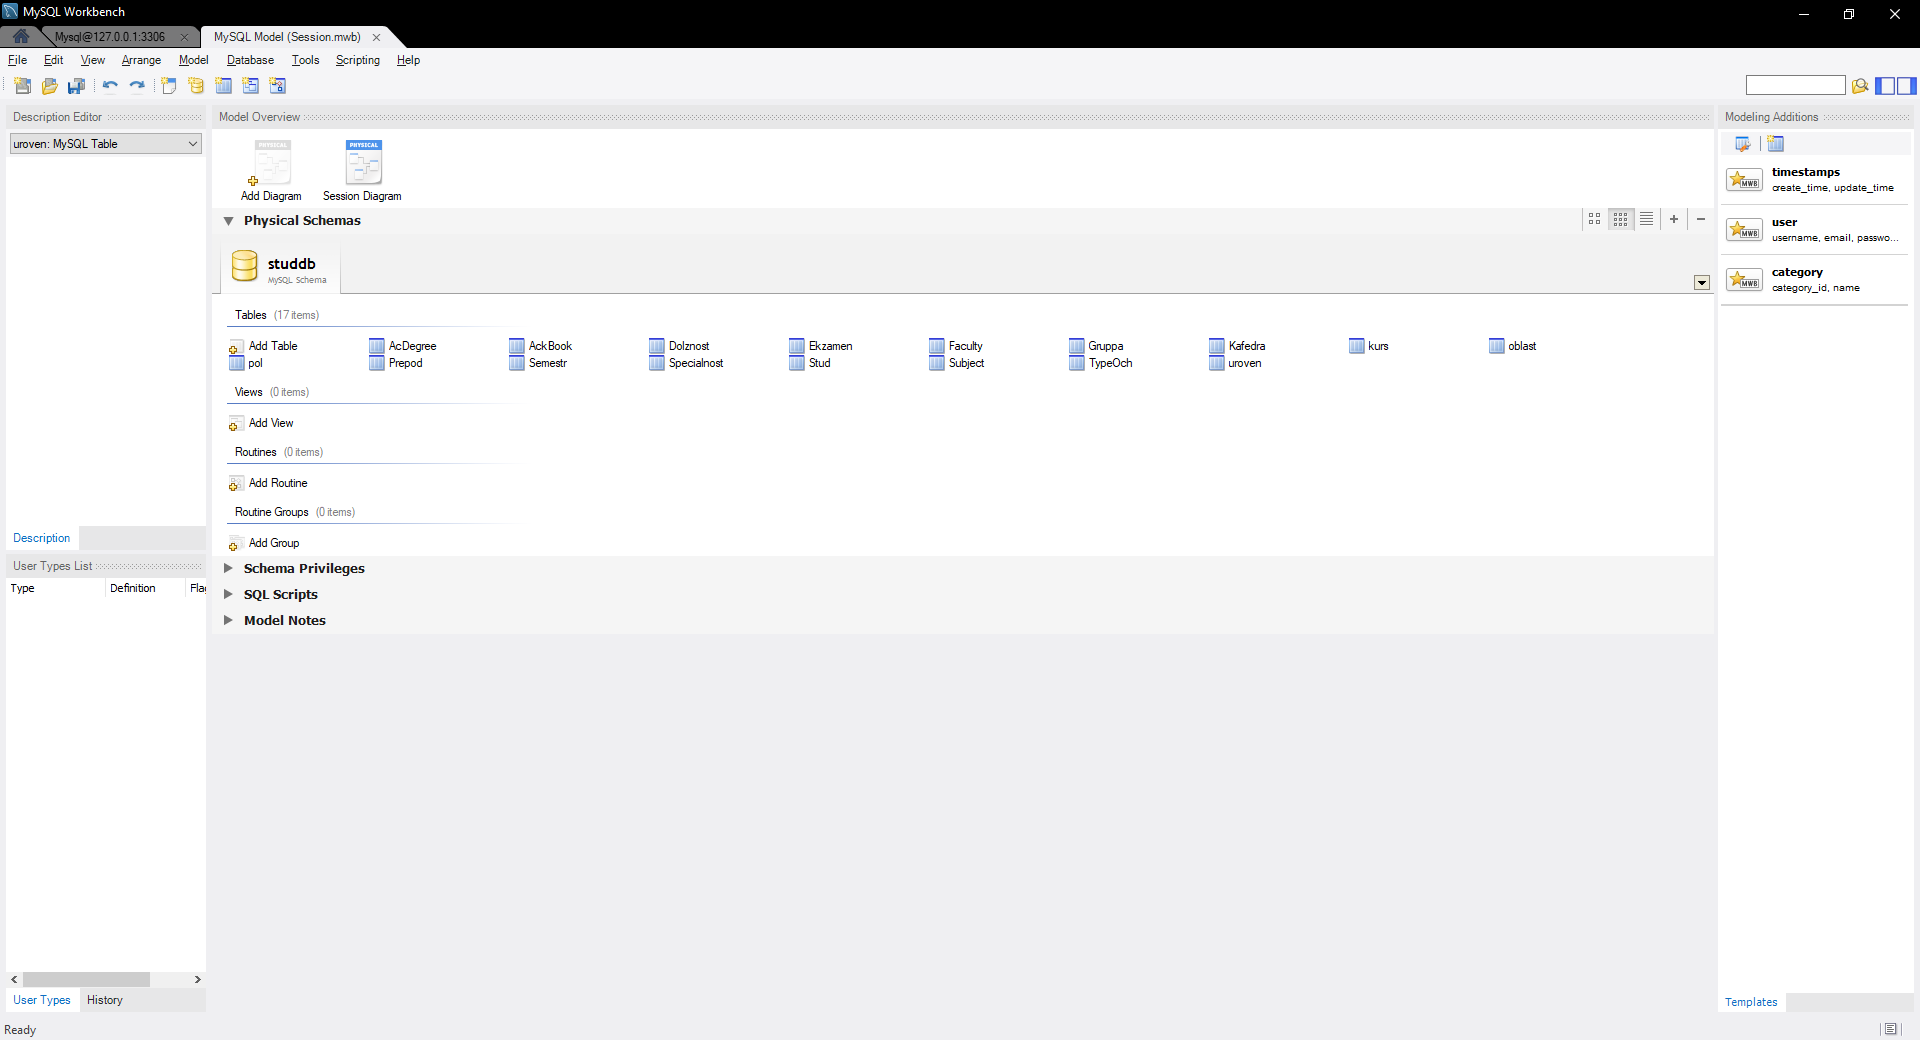
\includegraphics[width=\textwidth]{1.png}

\section{Информация о создании таблиц}
\subsection{AcDegree}
\begin{lstlisting}
CREATE TABLE IF NOT EXISTS `studdb`.`AcDegree` (
  `AcDegree_ID` INT NOT NULL,
  `fk_uroven_ID` VARCHAR(1) NULL,
  `fk_oblast_ID` INT NULL,
  `AcDegree` VARCHAR(50) NULL,
  `AcDegreeShort` VARCHAR(10) NULL,
  PRIMARY KEY (`AcDegree_ID`),
  INDEX `fk_oblast_ID_idx` (`fk_oblast_ID` ASC) VISIBLE,
  INDEX `fk_uroven_ID_idx` (`fk_uroven_ID` ASC) VISIBLE,
  CONSTRAINT `fk_uroven_ID`
    FOREIGN KEY (`fk_uroven_ID`)
    REFERENCES `studdb`.`uroven` (`uroven_id`)
    ON DELETE NO ACTION
    ON UPDATE NO ACTION,
  CONSTRAINT `fk_oblast_ID`
    FOREIGN KEY (`fk_oblast_ID`)
    REFERENCES `studdb`.`oblast` (`oblast_ID`)
    ON DELETE NO ACTION
    ON UPDATE NO ACTION)
ENGINE = InnoDB  
\end{lstlisting}
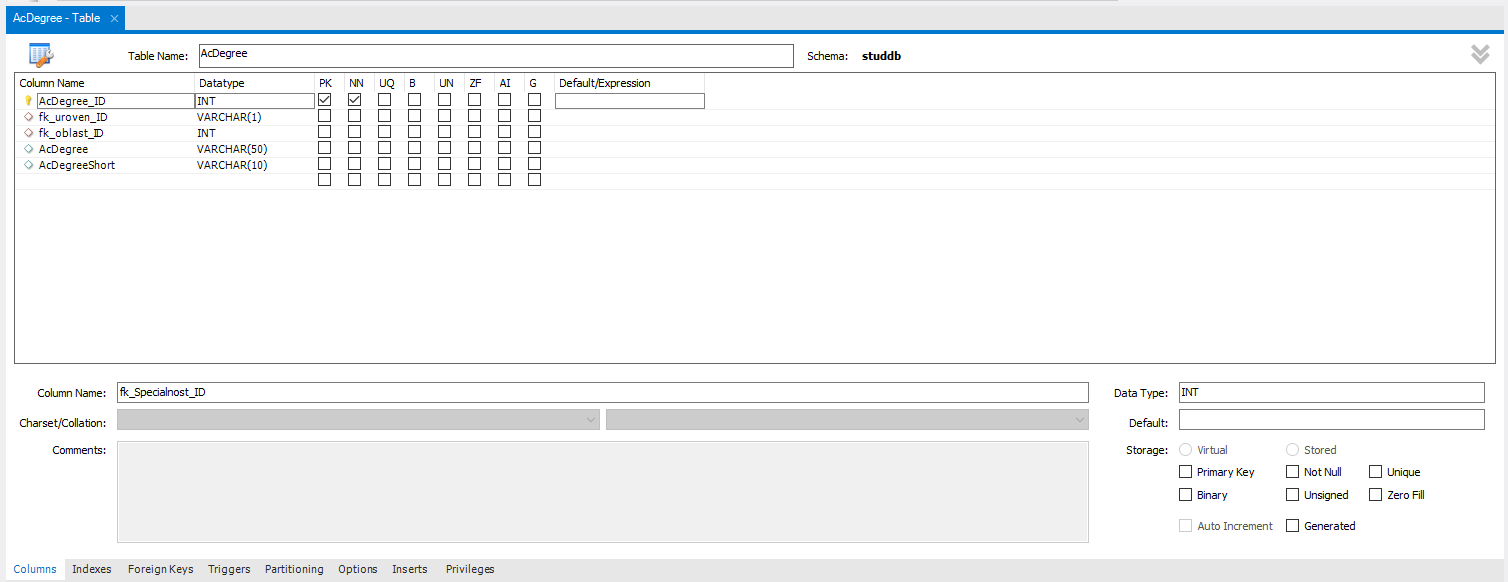
\includegraphics[width=\textwidth]{2-1.png}

\subsection{AckBook}
\begin{lstlisting}
CREATE TABLE IF NOT EXISTS `studdb`.`AckBook` (
  `AckBook_ID` INT NOT NULL,
  `fk_Ekzamen_ID` INT NULL,
  `fk_TypeOch_ID` INT NULL,
  `fk_Stud_ID` INT NULL,
  `DataRec` DATE NULL,
  PRIMARY KEY (`AckBook_ID`),
  INDEX `fk_Ekzamen_ID_idx` (`fk_Ekzamen_ID` ASC) VISIBLE,
  INDEX `fk_TypeOch_ID_idx` (`fk_TypeOch_ID` ASC) VISIBLE,
  INDEX `1_idx` (`fk_Stud_ID` ASC) VISIBLE,
  CONSTRAINT `fk_Ekzamen_ID`
    FOREIGN KEY (`fk_Ekzamen_ID`)
    REFERENCES `studdb`.`Ekzamen` (`Ekzamen_ID`)
    ON DELETE NO ACTION
    ON UPDATE NO ACTION,
  CONSTRAINT `fk_TypeOch_ID`
    FOREIGN KEY (`fk_TypeOch_ID`)
    REFERENCES `studdb`.`TypeOch` (`TypeOch_ID`)
    ON DELETE NO ACTION
    ON UPDATE NO ACTION,
  CONSTRAINT `fk_Stud_ID`
    FOREIGN KEY (`fk_Stud_ID`)
    REFERENCES `studdb`.`Stud` (`Stud_ID`)
    ON DELETE NO ACTION
    ON UPDATE NO ACTION)
ENGINE = InnoDB  
\end{lstlisting}
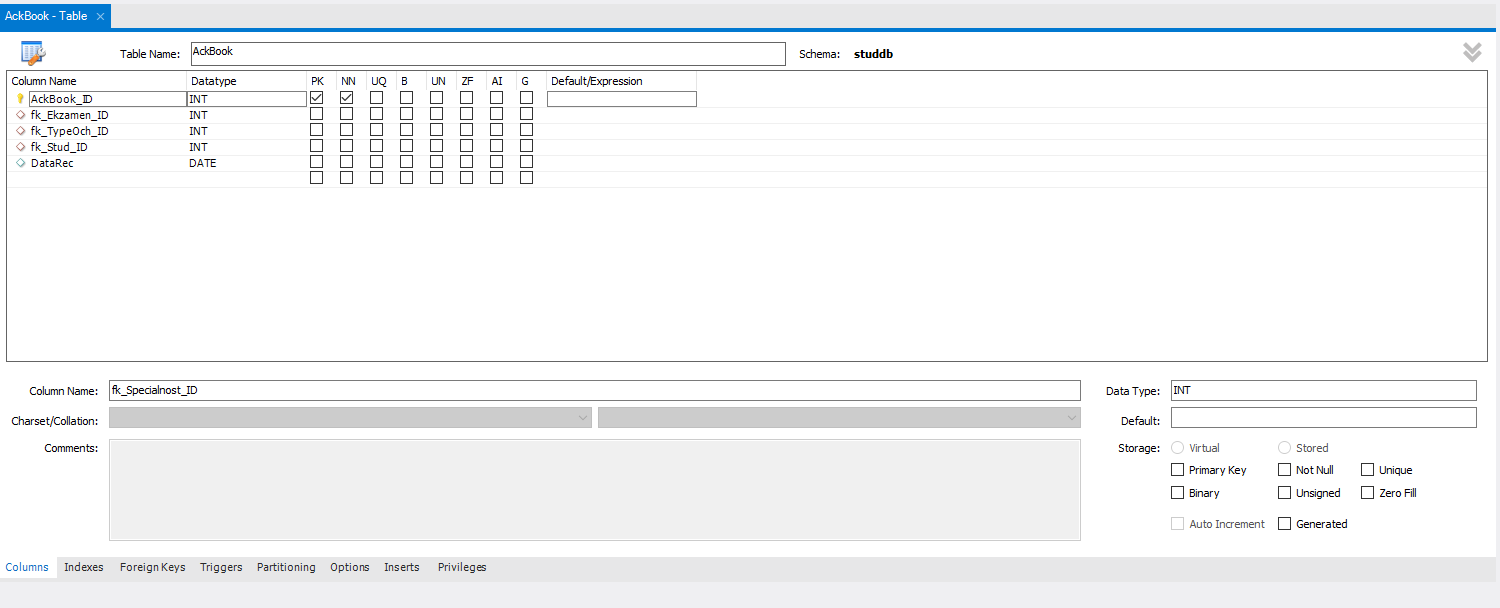
\includegraphics[width=\textwidth]{2-2.png}

\subsection{Dolznost}
\begin{lstlisting}
CREATE TABLE IF NOT EXISTS `studdb`.`Dolznost` (
  `Dolznost_ID` INT NOT NULL,
  `Dolznost` VARCHAR(20) NULL,
  PRIMARY KEY (`Dolznost_ID`))
ENGINE = InnoDB
\end{lstlisting}
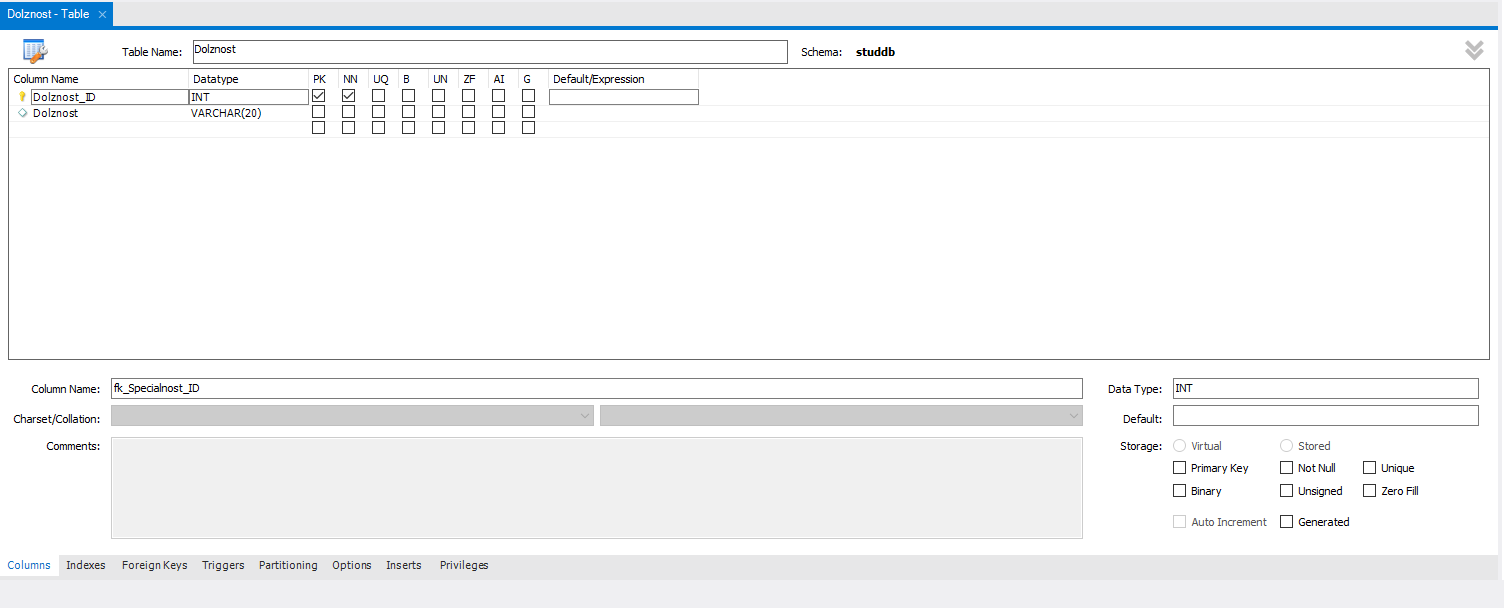
\includegraphics[width=\textwidth]{2-3.png}

\subsection{Ekzamen}
\begin{lstlisting}
CREATE TABLE IF NOT EXISTS `studdb`.`Ekzamen` (
  `Ekzamen_ID` INT NOT NULL,
  `fk_Specialnost_ID` INT NULL,
  `fk_Semestr_ID` INT NULL,
  `fk_Subject_ID` INT NULL,
  `fk_Prepod_ID` INT NULL,
  PRIMARY KEY (`Ekzamen_ID`),
  INDEX `fk_Specialnost_ID_idx` (`fk_Specialnost_ID` ASC) VISIBLE,
  INDEX `fk_Semestr_ID_idx` (`fk_Semestr_ID` ASC) VISIBLE,
  INDEX `fk_Subject_ID_idx` (`fk_Subject_ID` ASC) VISIBLE,
  INDEX `fk_Prepod_ID_idx` (`fk_Prepod_ID` ASC) VISIBLE,
  CONSTRAINT `fk_Specialnost_ID`
    FOREIGN KEY (`fk_Specialnost_ID`)
    REFERENCES `studdb`.`Specialnost` (`Specialnost_ID`)
    ON DELETE NO ACTION
    ON UPDATE NO ACTION,
  CONSTRAINT `fk_Semestr_ID`
    FOREIGN KEY (`fk_Semestr_ID`)
    REFERENCES `studdb`.`Semestr` (`Semestr_ID`)
    ON DELETE NO ACTION
    ON UPDATE NO ACTION,
  CONSTRAINT `fk_Subject_ID`
    FOREIGN KEY (`fk_Subject_ID`)
    REFERENCES `studdb`.`Subject` (`Subject_ID`)
    ON DELETE NO ACTION
    ON UPDATE NO ACTION,
  CONSTRAINT `fk_Prepod_ID`
    FOREIGN KEY (`fk_Prepod_ID`)
    REFERENCES `studdb`.`Prepod` (`Prepod_ID`)
    ON DELETE NO ACTION
    ON UPDATE NO ACTION)
ENGINE = InnoDB  
\end{lstlisting}
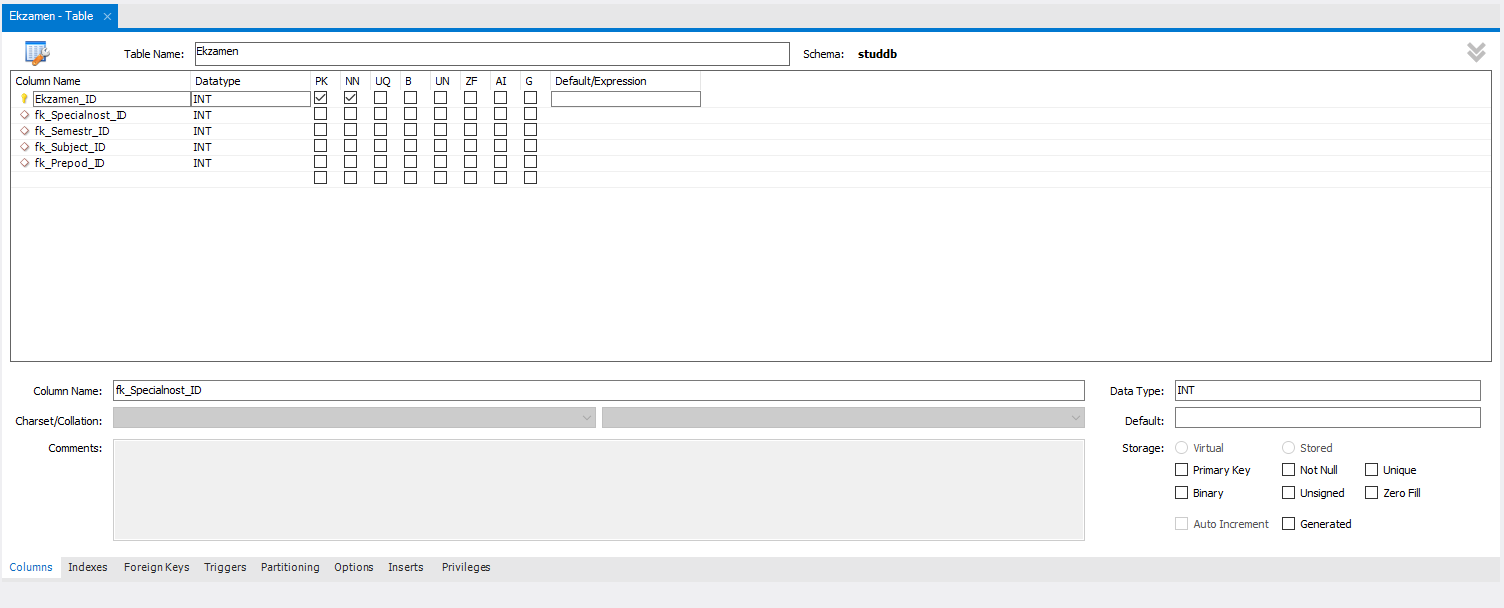
\includegraphics[width=\textwidth]{2-4.png}

\subsection{Faculty}
\begin{lstlisting}
 CREATE TABLE IF NOT EXISTS `studdb`.`Faculty` (
  `Faculty_ID` INT NOT NULL,
  `Faculty` VARCHAR(40) NULL,
  `FacShort` VARCHAR(6) NULL,
  PRIMARY KEY (`Faculty_ID`))
ENGINE = InnoDB 
\end{lstlisting}
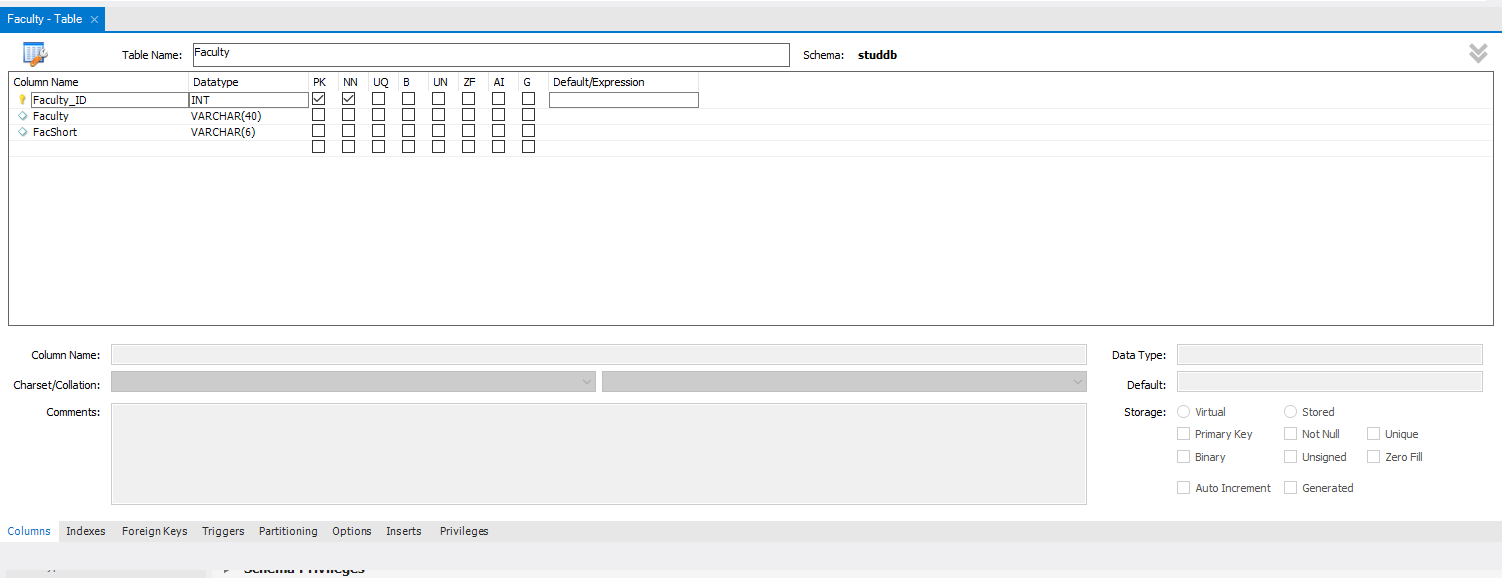
\includegraphics[width=\textwidth]{2-5.png}

\subsection{Gruppa}
\begin{lstlisting}
CREATE TABLE IF NOT EXISTS `studdb`.`Gruppa` (
  `Gruppa_ID` INT NOT NULL,
  `fk_Faculty_ID` INT NULL,
  `fk_kurs_ID` INT NULL,
  `fk_Specialnost_ID` INT NULL,
  `Gruppa` VARCHAR(10) NULL,
  PRIMARY KEY (`Gruppa_ID`),
  INDEX `fk_Faculty_ID_idx` (`fk_Faculty_ID` ASC) VISIBLE,
  INDEX `fk_kurs_ID_idx` (`fk_kurs_ID` ASC) VISIBLE,
  INDEX `fk_Specialnost_ID_idx` (`fk_Specialnost_ID` ASC) VISIBLE,
  CONSTRAINT `fk_Faculty_ID`
    FOREIGN KEY (`fk_Faculty_ID`)
    REFERENCES `studdb`.`Faculty` (`Faculty_ID`)
    ON DELETE NO ACTION
    ON UPDATE NO ACTION,
  CONSTRAINT `fk_kurs_ID`
    FOREIGN KEY (`fk_kurs_ID`)
    REFERENCES `studdb`.`kurs` (`kurs_ID`)
    ON DELETE NO ACTION
    ON UPDATE NO ACTION,
  CONSTRAINT `fk_Specialnost_ID`
    FOREIGN KEY (`fk_Specialnost_ID`)
    REFERENCES `studdb`.`Specialnost` (`Specialnost_ID`)
    ON DELETE NO ACTION
    ON UPDATE NO ACTION)
ENGINE = InnoDB  
\end{lstlisting}
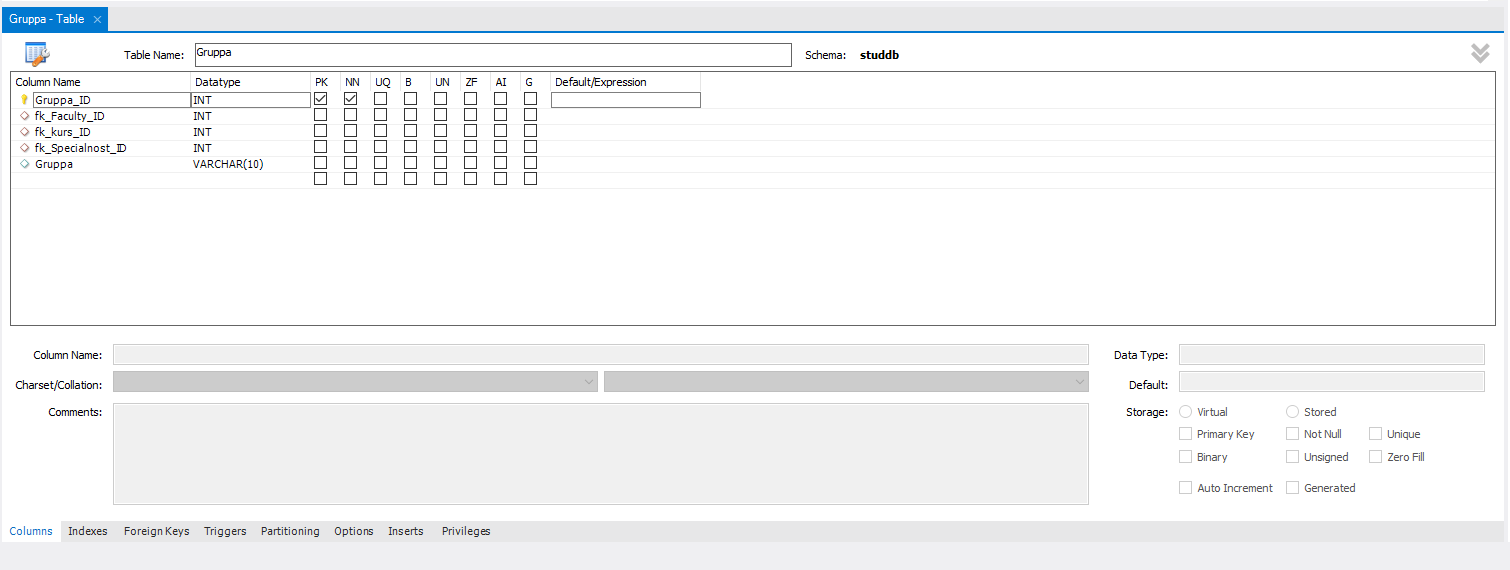
\includegraphics[width=\textwidth]{2-6.png}

\subsection{Kafedra}
\begin{lstlisting}
 CREATE TABLE IF NOT EXISTS `studdb`.`Kafedra` (
  `Kafedra_ID` INT NOT NULL,
  `Kafedra` VARCHAR(50) NULL,
  `KafedraShort` VARCHAR(10) NULL,
  PRIMARY KEY (`Kafedra_ID`))
ENGINE = InnoDB 
\end{lstlisting}
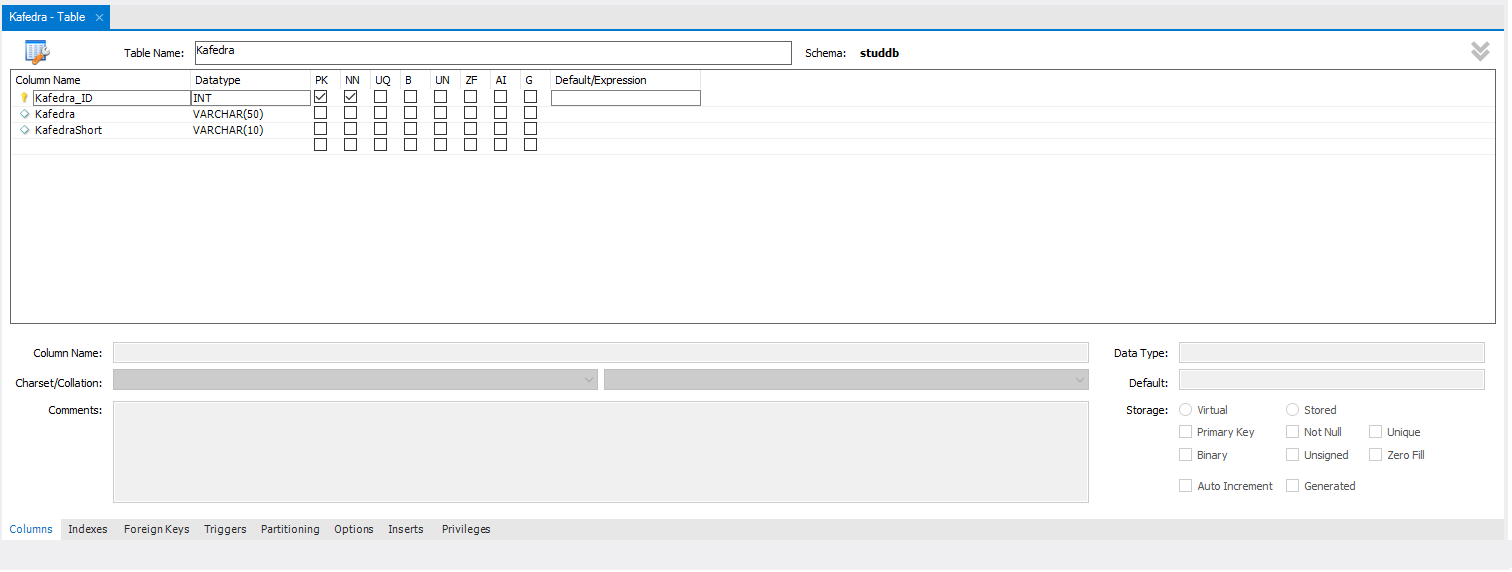
\includegraphics[width=\textwidth]{2-7.png}

\subsection{kurs}
\begin{lstlisting}
 CREATE TABLE IF NOT EXISTS `studdb`.`kurs` (
  `kurs_ID` INT NOT NULL,
  PRIMARY KEY (`kurs_ID`))
ENGINE = InnoDB 
\end{lstlisting}
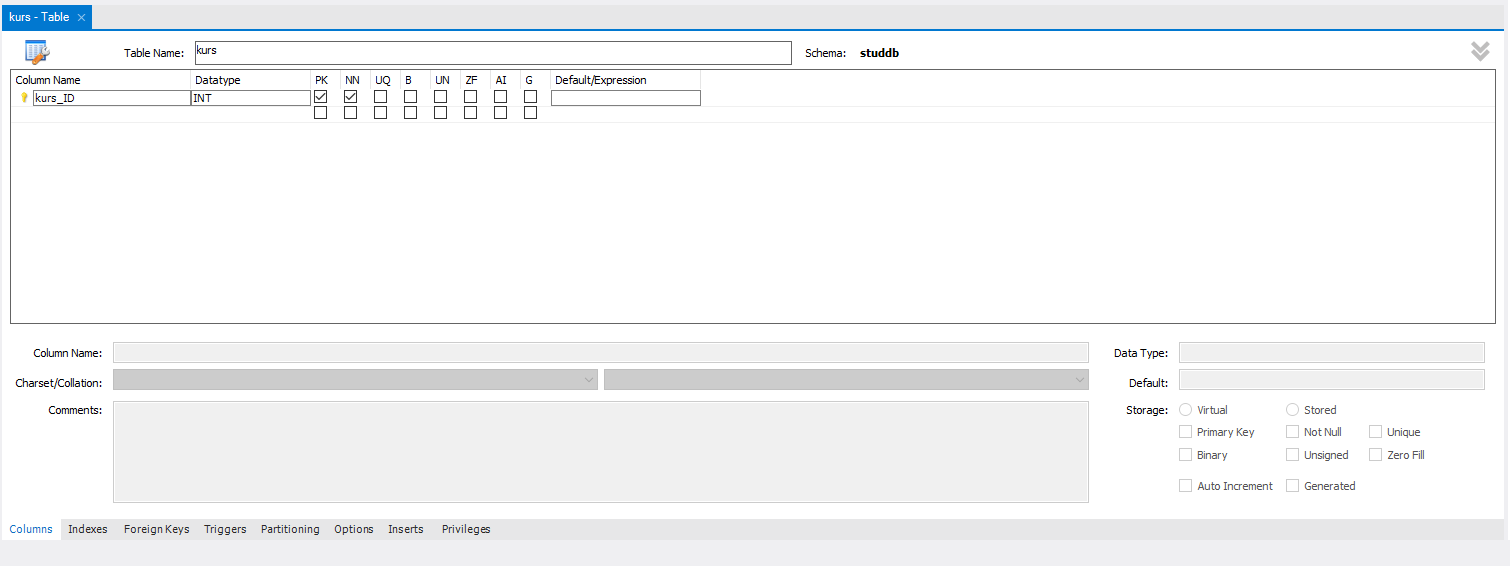
\includegraphics[width=\textwidth]{2-8.png}

\subsection{oblast}
\begin{lstlisting}
 CREATE TABLE IF NOT EXISTS `studdb`.`oblast` (
  `oblast_ID` INT NOT NULL,
  `oblast` VARCHAR(30) NULL,
  PRIMARY KEY (`oblast_ID`))
ENGINE = InnoDB 
\end{lstlisting}
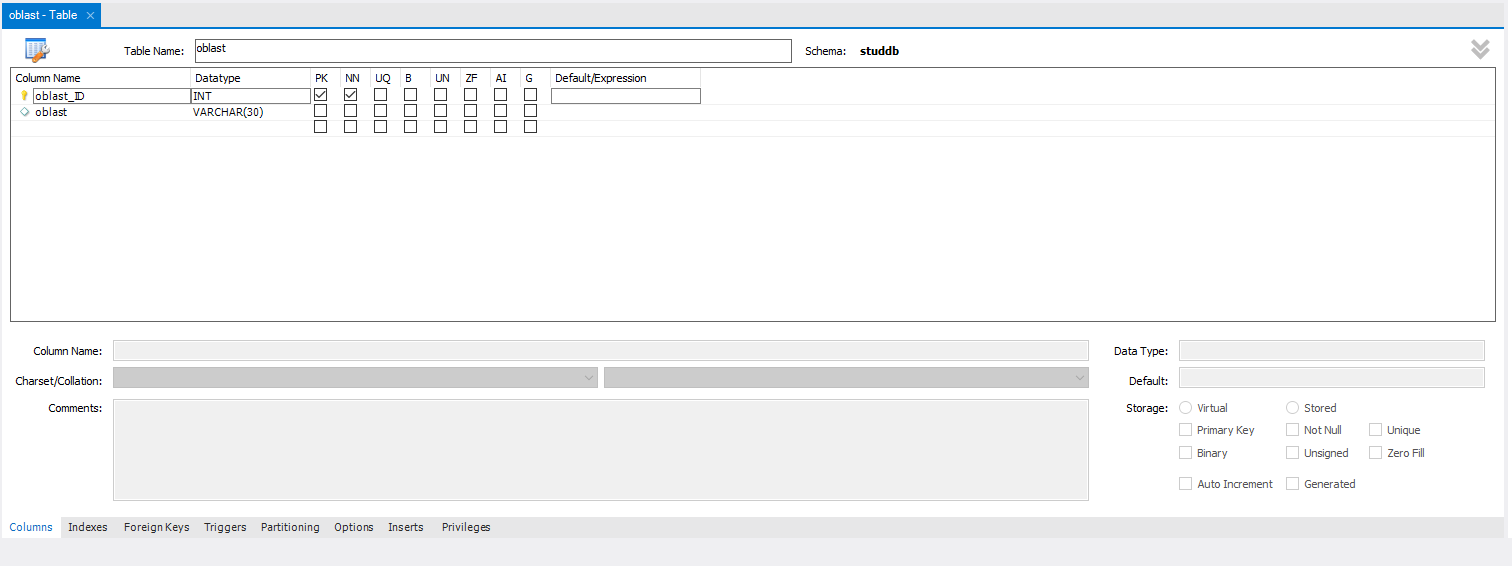
\includegraphics[width=\textwidth]{2-9.png}

\subsection{pol}
\begin{lstlisting}
 CREATE TABLE IF NOT EXISTS `studdb`.`pol` (
  `pol_id` INT NOT NULL,
  `pol` VARCHAR(7) NULL,
  `pol_short` VARCHAR(1) NULL,
  PRIMARY KEY (`pol_id`))
ENGINE = InnoDB 
\end{lstlisting}
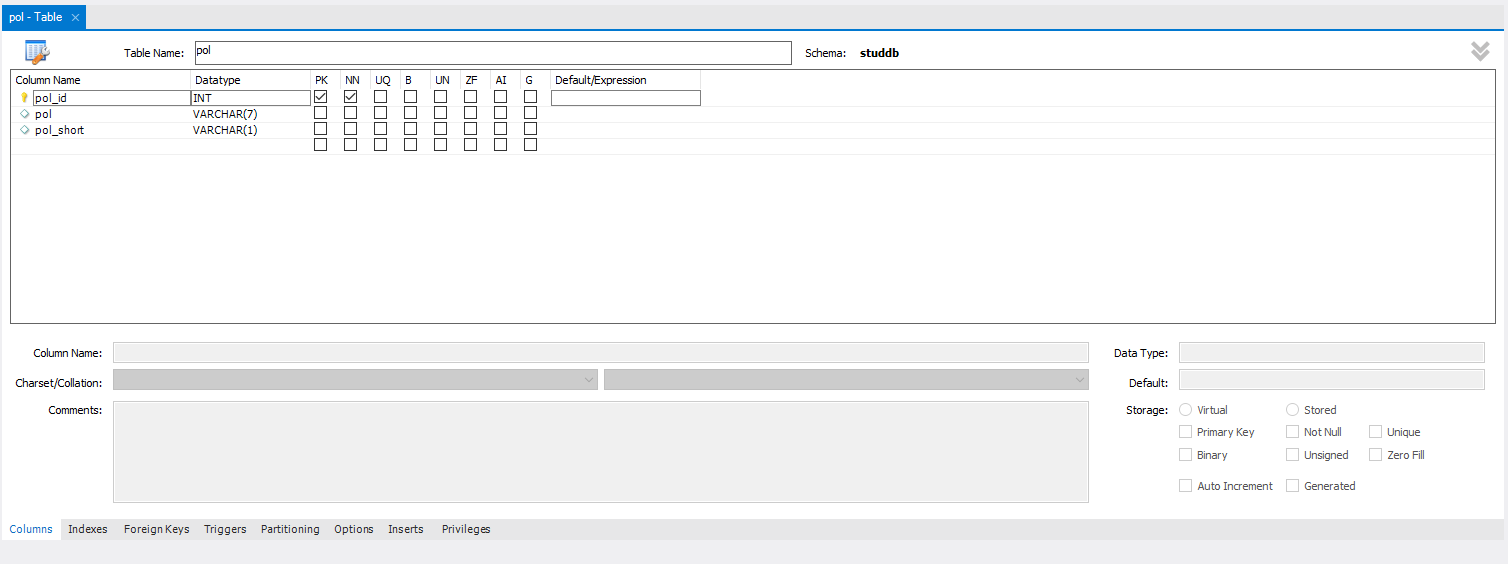
\includegraphics[width=\textwidth]{2-10.png}

\subsection{Prepod}
\begin{lstlisting}
 CREATE TABLE IF NOT EXISTS `studdb`.`Prepod` (
  `Prepod_ID` INT NOT NULL,
  `fk_Dolznost_ID` INT NULL,
  `fk_AcDegree_ID` INT NULL,
  `fk_Kafedra_ID` INT NULL,
  `LName` VARCHAR(50) NULL,
  `FName` VARCHAR(50) NULL,
  `MName` VARCHAR(50) NULL,
  `BirthDay` DATE NULL,
  PRIMARY KEY (`Prepod_ID`),
  INDEX `fk_Dolznost_ID_idx` (`fk_Dolznost_ID` ASC) VISIBLE,
  INDEX `fk_AcDegree_ID_idx` (`fk_AcDegree_ID` ASC) VISIBLE,
  INDEX `fk_Kafedra_ID_idx` (`fk_Kafedra_ID` ASC) VISIBLE,
  CONSTRAINT `fk_Dolznost_ID`
    FOREIGN KEY (`fk_Dolznost_ID`)
    REFERENCES `studdb`.`Dolznost` (`Dolznost_ID`)
    ON DELETE NO ACTION
    ON UPDATE NO ACTION,
  CONSTRAINT `fk_AcDegree_ID`
    FOREIGN KEY (`fk_AcDegree_ID`)
    REFERENCES `studdb`.`AcDegree` (`AcDegree_ID`)
    ON DELETE NO ACTION
    ON UPDATE NO ACTION,
  CONSTRAINT `fk_Kafedra_ID`
    FOREIGN KEY (`fk_Kafedra_ID`)
    REFERENCES `studdb`.`Kafedra` (`Kafedra_ID`)
    ON DELETE NO ACTION
    ON UPDATE NO ACTION)
ENGINE = InnoDB 
\end{lstlisting}
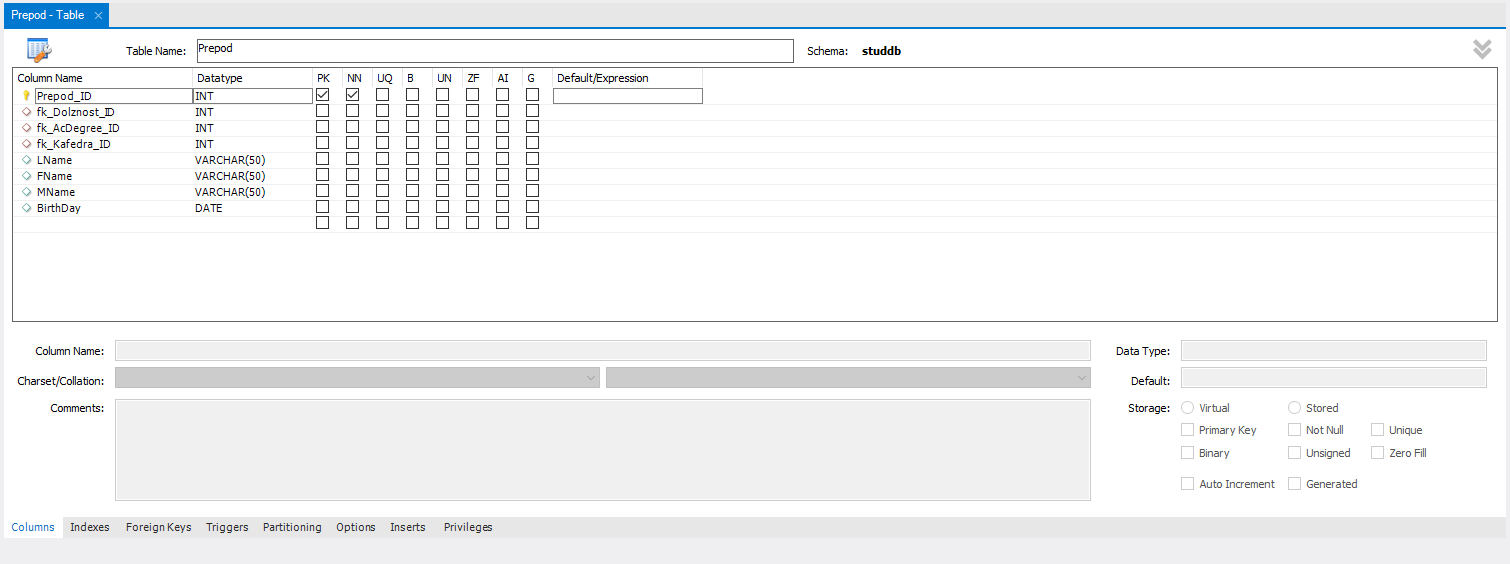
\includegraphics[width=\textwidth]{2-11.png}

\subsection{Semestr}
\begin{lstlisting}
 CREATE TABLE IF NOT EXISTS `studdb`.`Semestr` (
  `Semestr_ID` INT NOT NULL,
  `fk_kurs_ID` INT NULL,
  `Semestr` INT NULL,
  PRIMARY KEY (`Semestr_ID`),
  INDEX `fk_kurs_ID_idx` (`fk_kurs_ID` ASC) VISIBLE,
  CONSTRAINT `fk_kurs_ID`
    FOREIGN KEY (`fk_kurs_ID`)
    REFERENCES `studdb`.`kurs` (`kurs_ID`)
    ON DELETE NO ACTION
    ON UPDATE NO ACTION)
ENGINE = InnoDB 
\end{lstlisting}
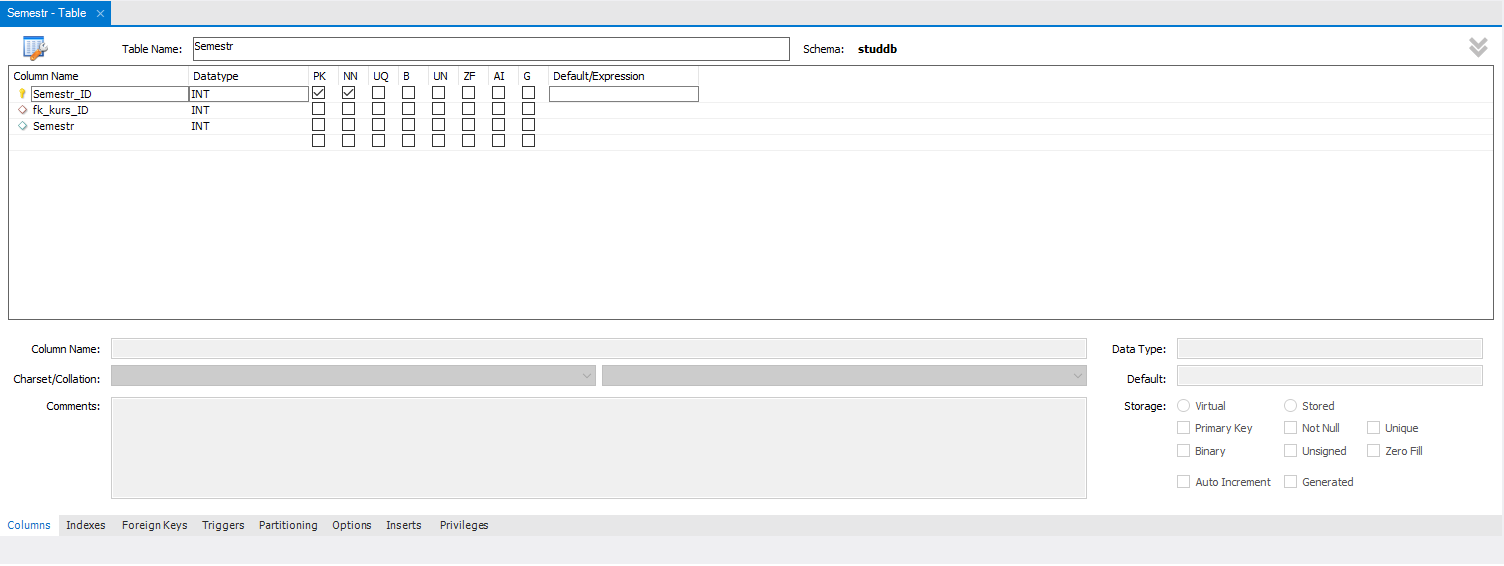
\includegraphics[width=\textwidth]{2-12.png}

\subsection{Specialnost}
\begin{lstlisting}
 CREATE TABLE IF NOT EXISTS `studdb`.`Specialnost` (
  `Specialnost_ID` INT NOT NULL,
  `Specialnost` VARCHAR(100) NULL,
  `CodOCSO` VARCHAR(10) NULL,
  PRIMARY KEY (`Specialnost_ID`))
ENGINE = InnoDB 
\end{lstlisting}
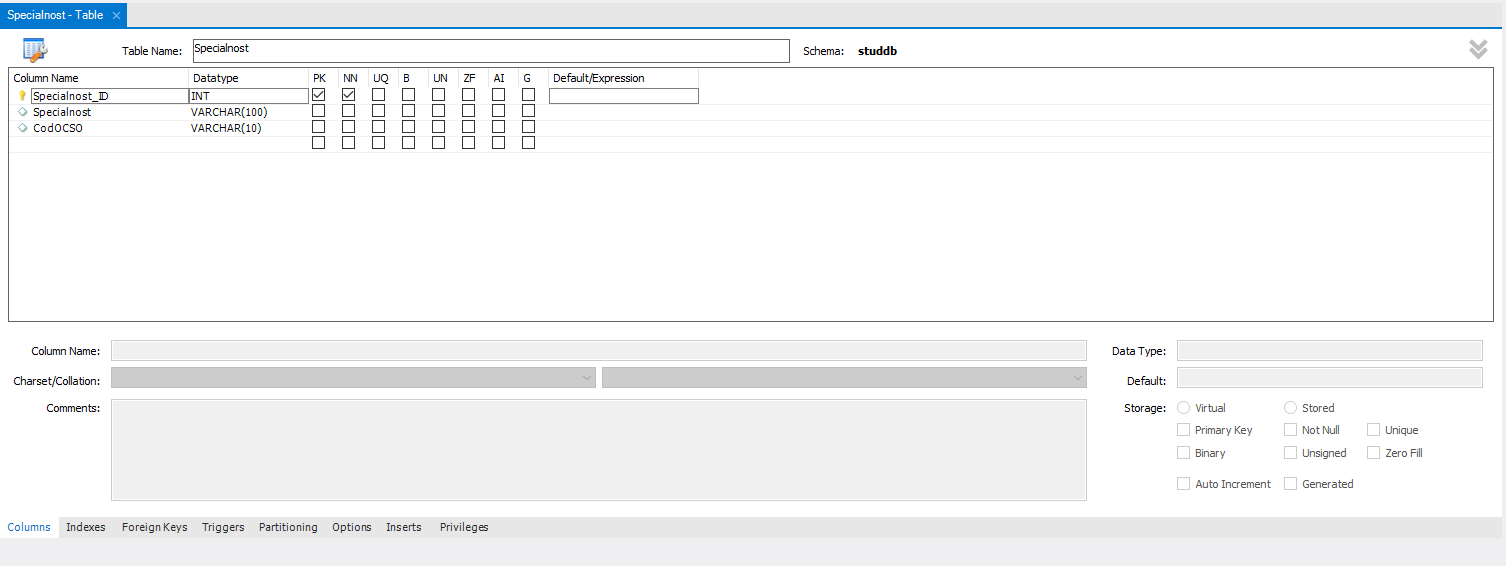
\includegraphics[width=\textwidth]{2-13.png}

\subsection{Stud}
\begin{lstlisting}
 CREATE TABLE IF NOT EXISTS `studdb`.`Stud` (
  `Stud_ID` INT NOT NULL,
  `fk_pol_id` INT NULL,
  `fk_Gruppa_ID` INT NULL,
  `NoZach` VARCHAR(10) NULL,
  `LName` VARCHAR(50) NULL,
  `FName` VARCHAR(50) NULL,
  `MName` VARCHAR(50) NULL,
  `BirthDay` DATE NULL,
  `Rost` DECIMAL(7,2) NULL,
  `Ves` INT NULL,
  `Stipendia` INT NULL,
  PRIMARY KEY (`Stud_ID`),
  INDEX `fk_pol_id_idx` (`fk_pol_id` ASC) VISIBLE,
  INDEX `fk_Gruppa_ID_idx` (`fk_Gruppa_ID` ASC) VISIBLE,
  CONSTRAINT `fk_pol_id`
    FOREIGN KEY (`fk_pol_id`)
    REFERENCES `studdb`.`pol` (`pol_id`)
    ON DELETE NO ACTION
    ON UPDATE NO ACTION,
  CONSTRAINT `fk_Gruppa_ID`
    FOREIGN KEY (`fk_Gruppa_ID`)
    REFERENCES `studdb`.`Gruppa` (`Gruppa_ID`)
    ON DELETE NO ACTION
    ON UPDATE NO ACTION)
ENGINE = InnoDB 
\end{lstlisting}
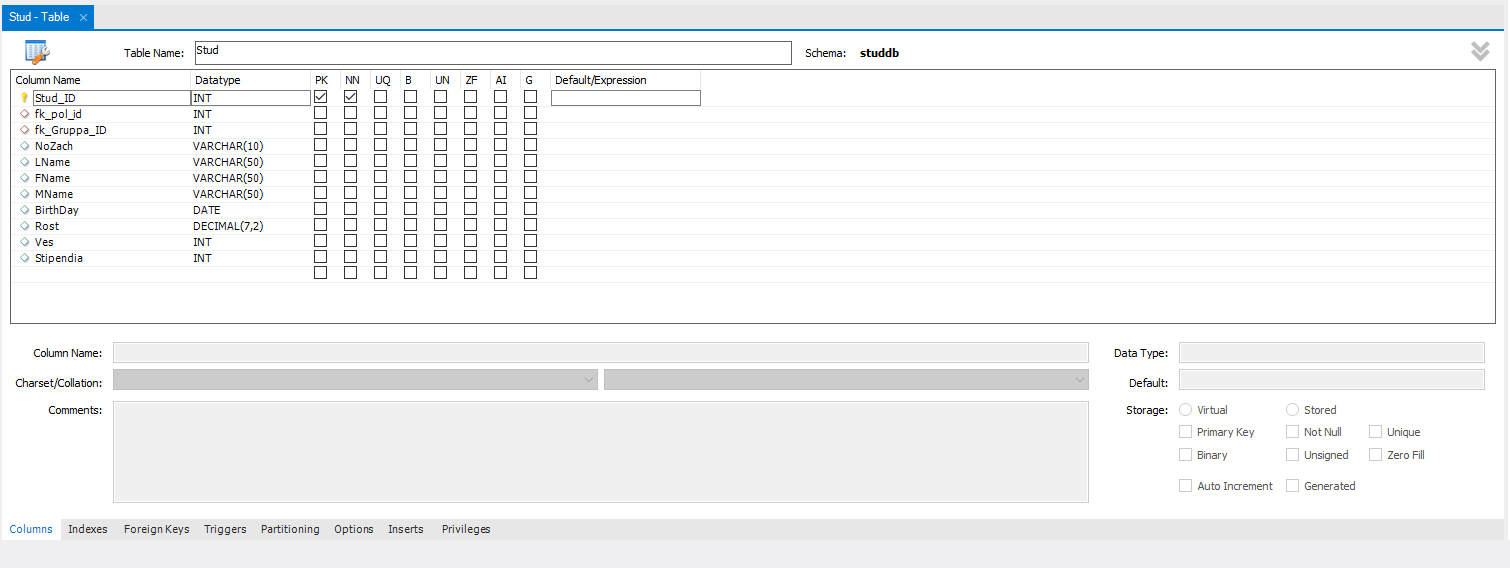
\includegraphics[width=\textwidth]{2-14.png}

\subsection{Subject}
\begin{lstlisting}
 CREATE TABLE IF NOT EXISTS `studdb`.`Subject` (
  `Subject_ID` INT NOT NULL,
  `Subject` VARCHAR(50) NULL,
  `ShortSubject` VARCHAR(10) NULL,
  PRIMARY KEY (`Subject_ID`))
ENGINE = InnoDB 
\end{lstlisting}
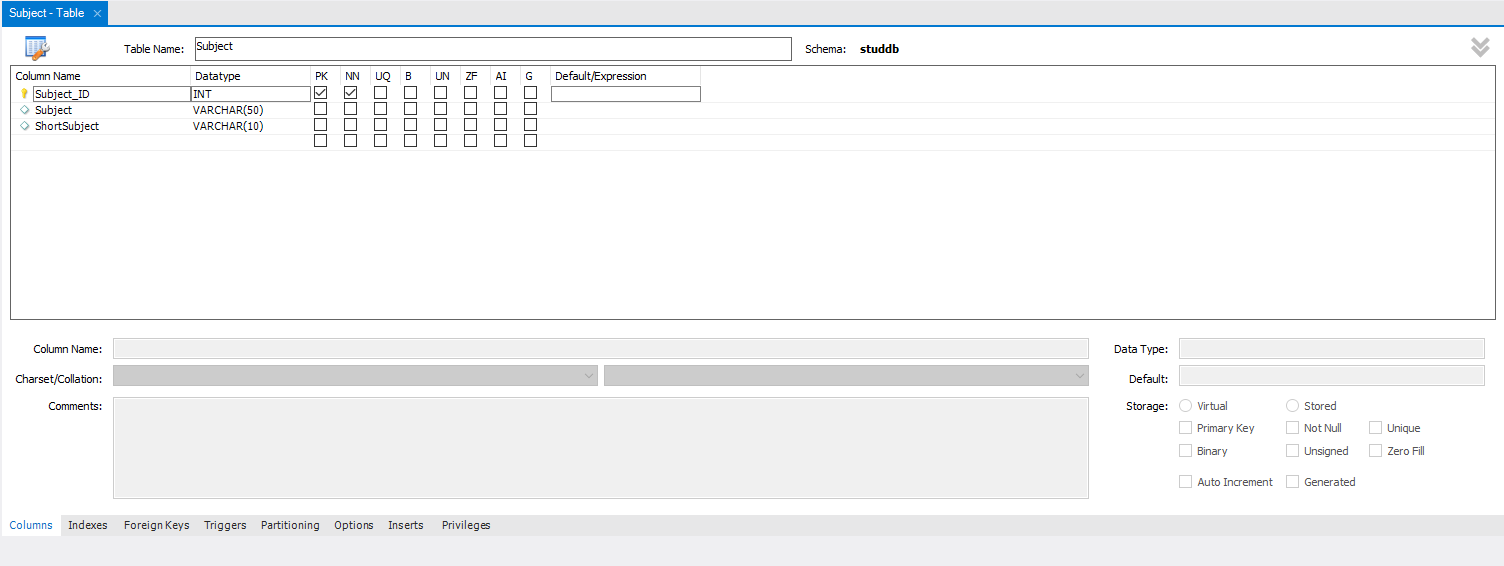
\includegraphics[width=\textwidth]{2-15.png}

\subsection{TypeOch}
\begin{lstlisting}
 CREATE TABLE IF NOT EXISTS `studdb`.`TypeOch` (
  `TypeOch_ID` INT NOT NULL,
  `TypeOch` INT NULL,
  `Coment` VARCHAR(20) NULL,
  PRIMARY KEY (`TypeOch_ID`))
ENGINE = InnoDB 
\end{lstlisting}
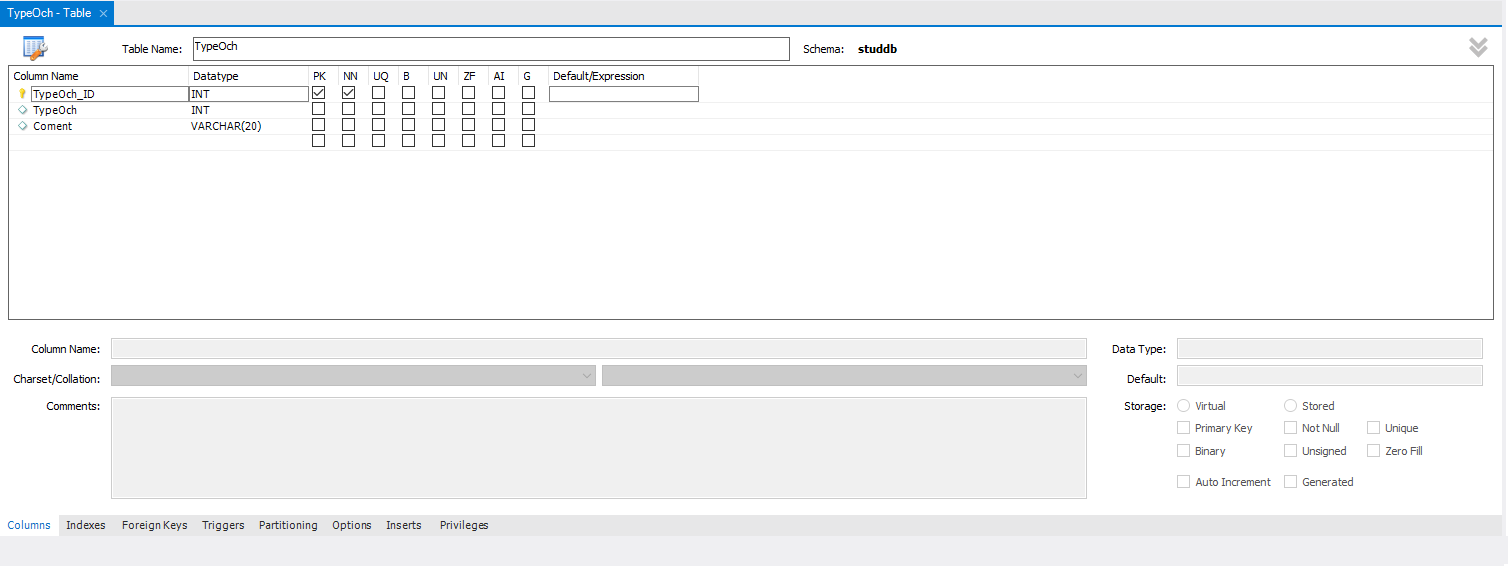
\includegraphics[width=\textwidth]{2-16.png}

\subsection{uroven}
\begin{lstlisting}
 CREATE TABLE IF NOT EXISTS `studdb`.`uroven` (
  `uroven_id` VARCHAR(1) NOT NULL,
  `uroven` VARCHAR(50) NULL,
  PRIMARY KEY (`uroven_id`))
ENGINE = InnoDB 
\end{lstlisting}
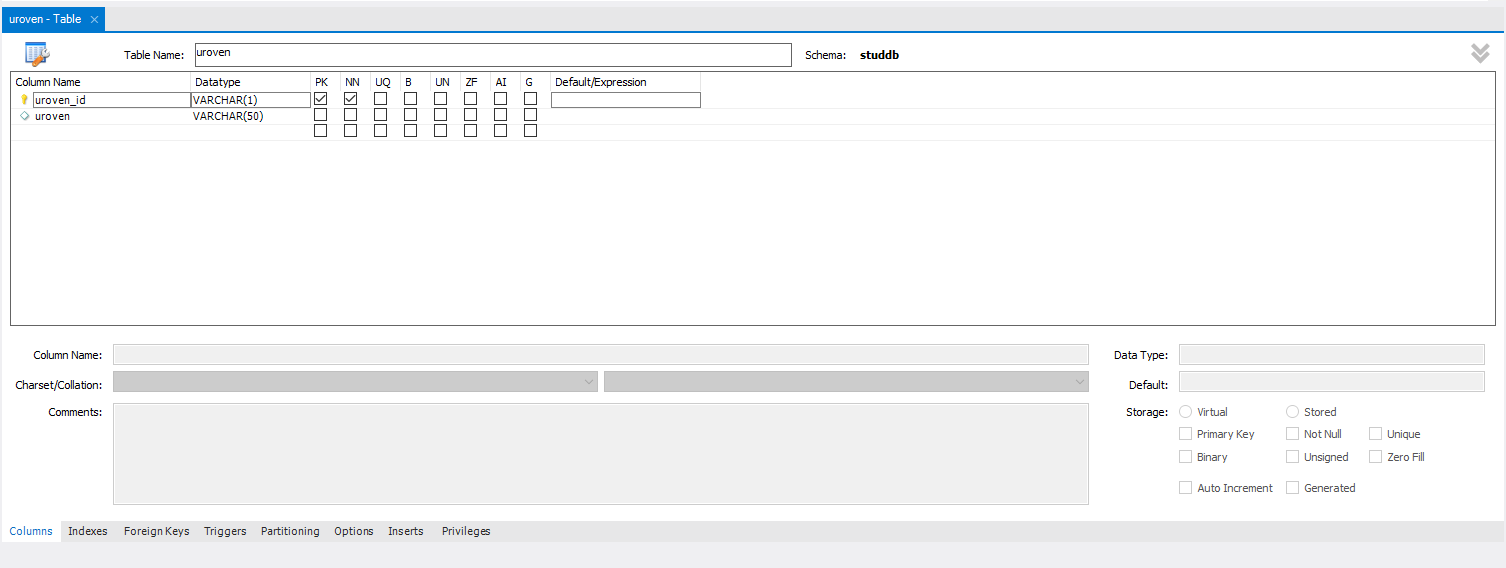
\includegraphics[width=\textwidth]{2-17.png}

\newpage
\section{Информация о создании ER-диаграммы}
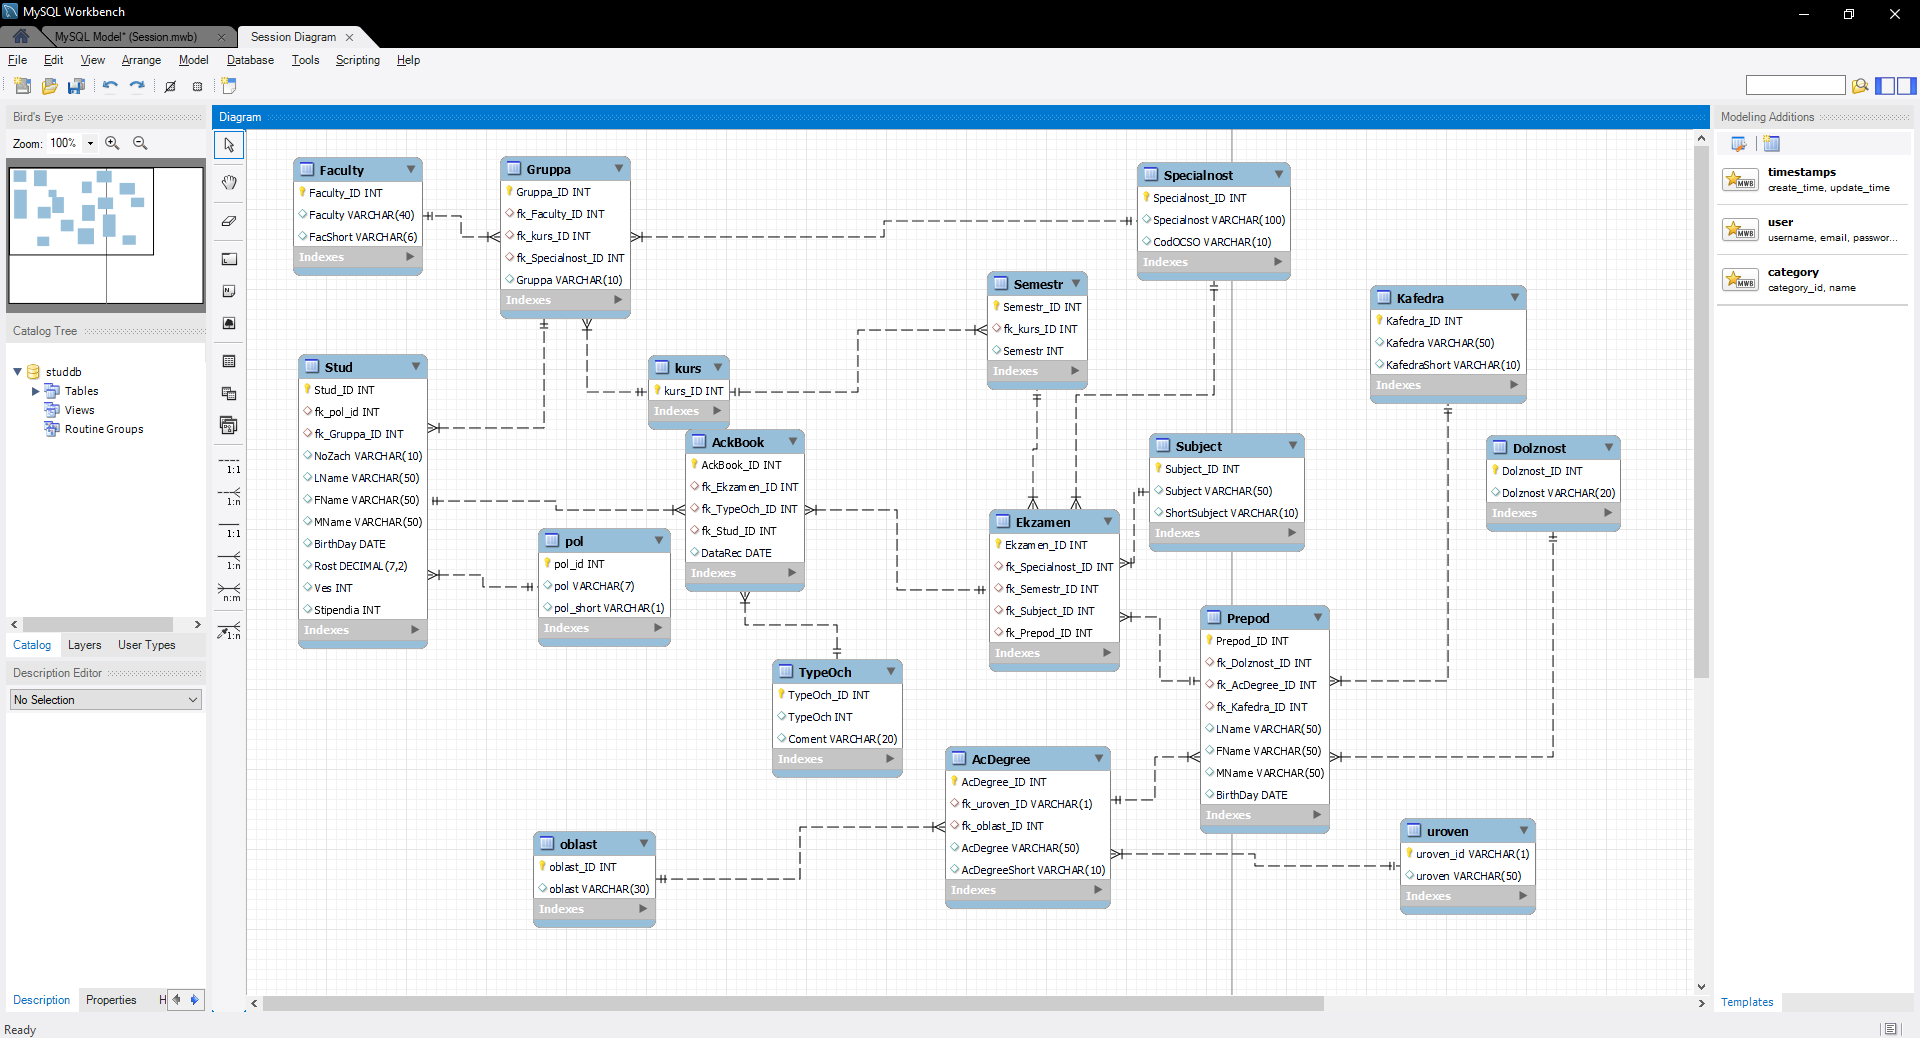
\includegraphics[width=\textwidth]{3.png}

\section{Информация о заполнении таблиц данными}
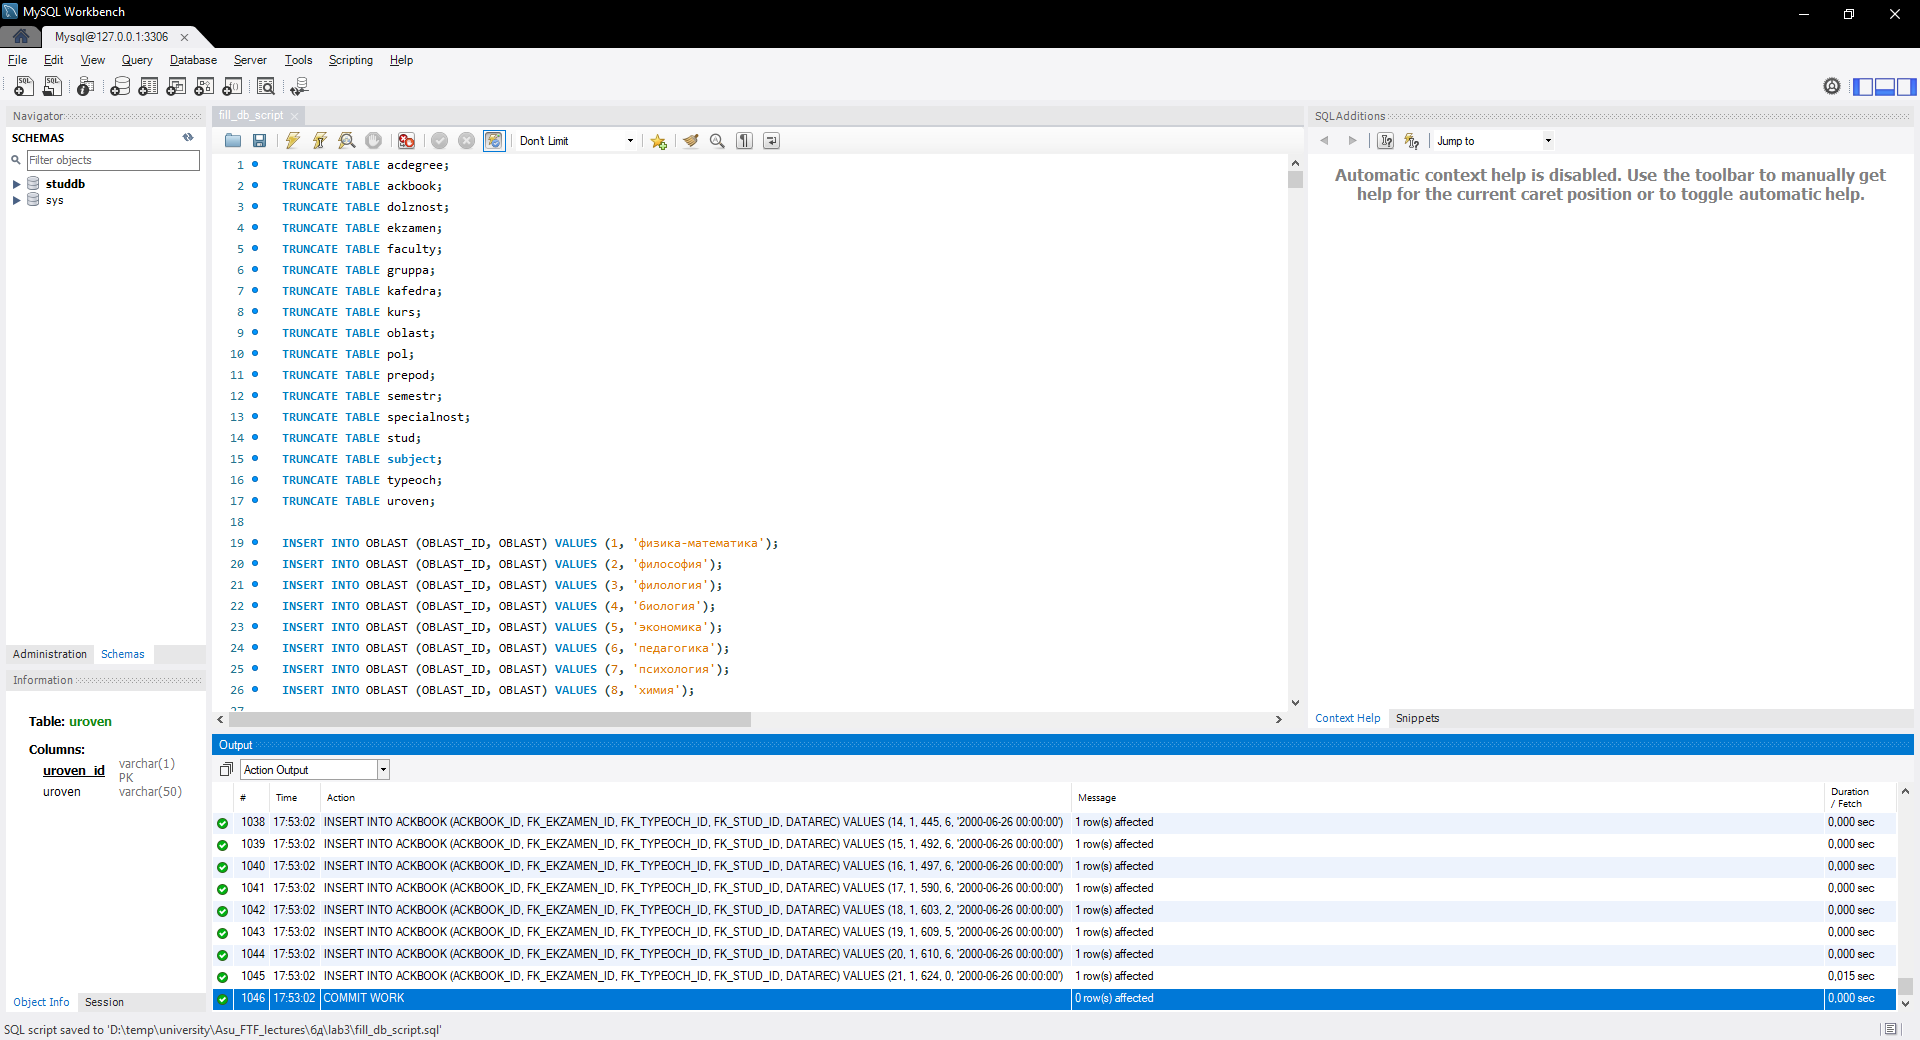
\includegraphics[width=\textwidth]{4.png}

\newpage
\section{Информация о результаты выполнения запросов}
\subsection{Вывести фамилии, имена и даты рождения всех девушек, родившихся в понедельник в январе.}
\begin{lstlisting}
select LName, FName, BirthDay from studdb.stud where dayofweek(BirthDay) = 2 and dayofmonth(BirthDay) = 1 and fk_pol_id = 0;
\end{lstlisting}
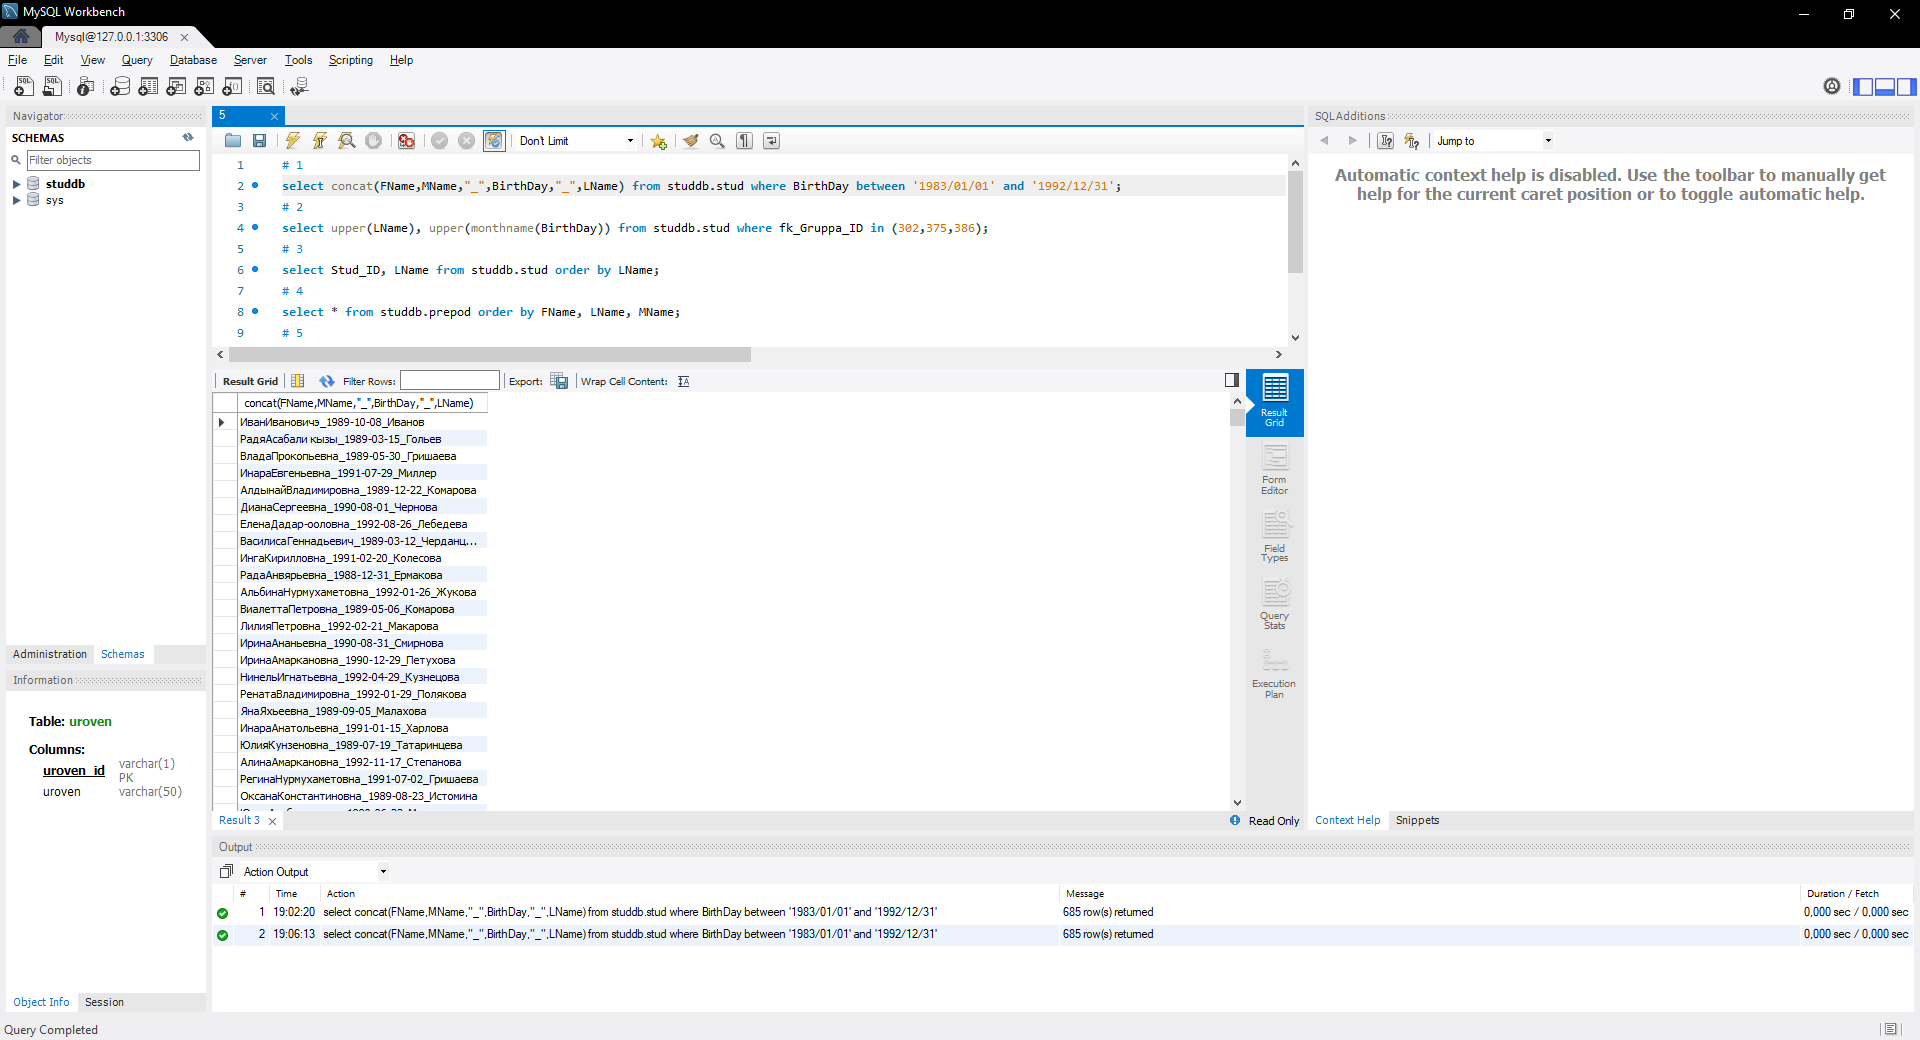
\includegraphics[width=\textwidth]{5-1.png}

\subsection{Вывести  фамилии и даты рождения всех юношей, родившихся в мае, сентябре и августе, у которых либо фамилии начинаются на А, либо содержат букву ж.}
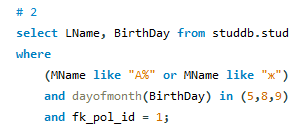
\includegraphics{5-2-1.png}\\
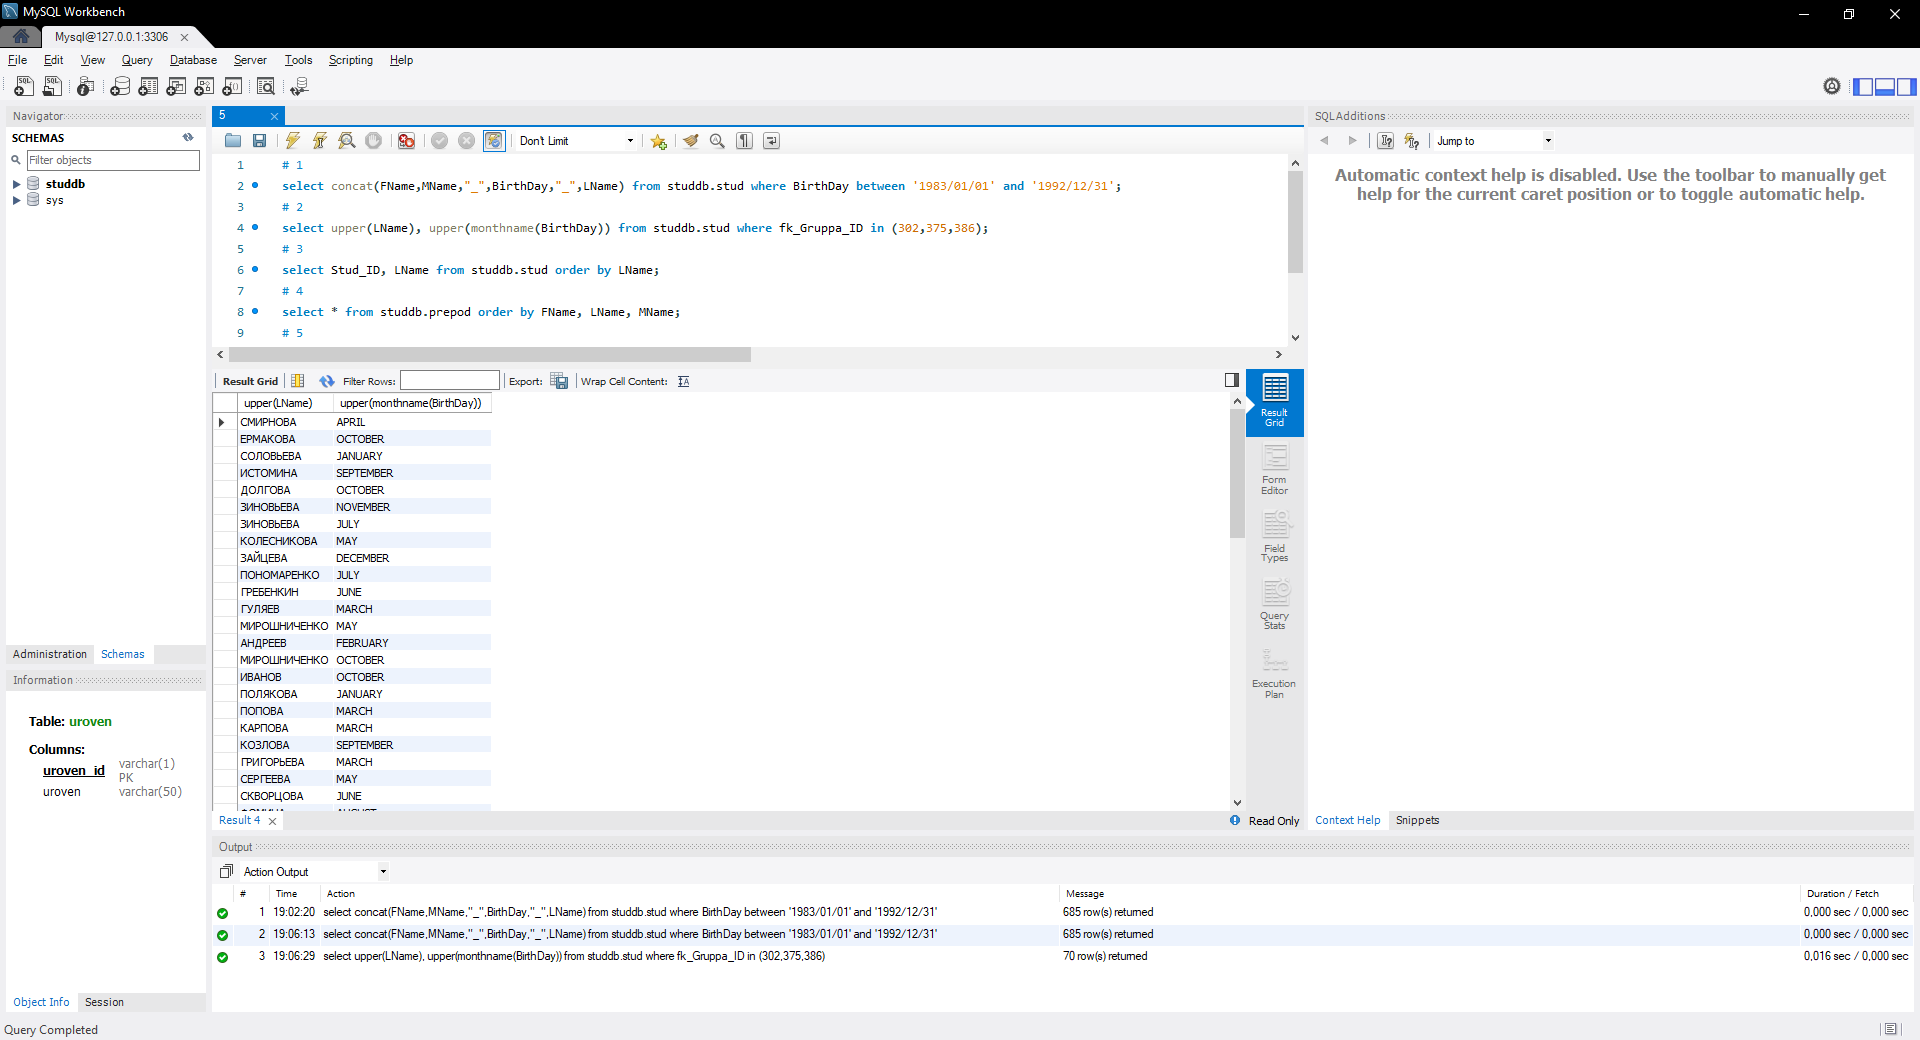
\includegraphics[width=\textwidth]{5-2.png}

\subsection{Вывести ФИО,  номер зачетки и дату рождения студентов (в формате «ФИО, № зачетки, дата рождения». Пример: Иванов Иван Иванович,  № 3256897855,  21.10.1991), которые родились осенью и младше 34 лет.}
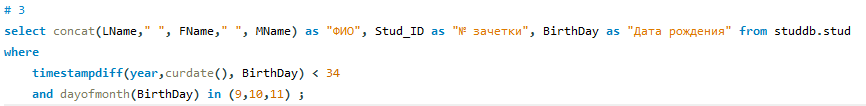
\includegraphics{5-3-1.png}\\
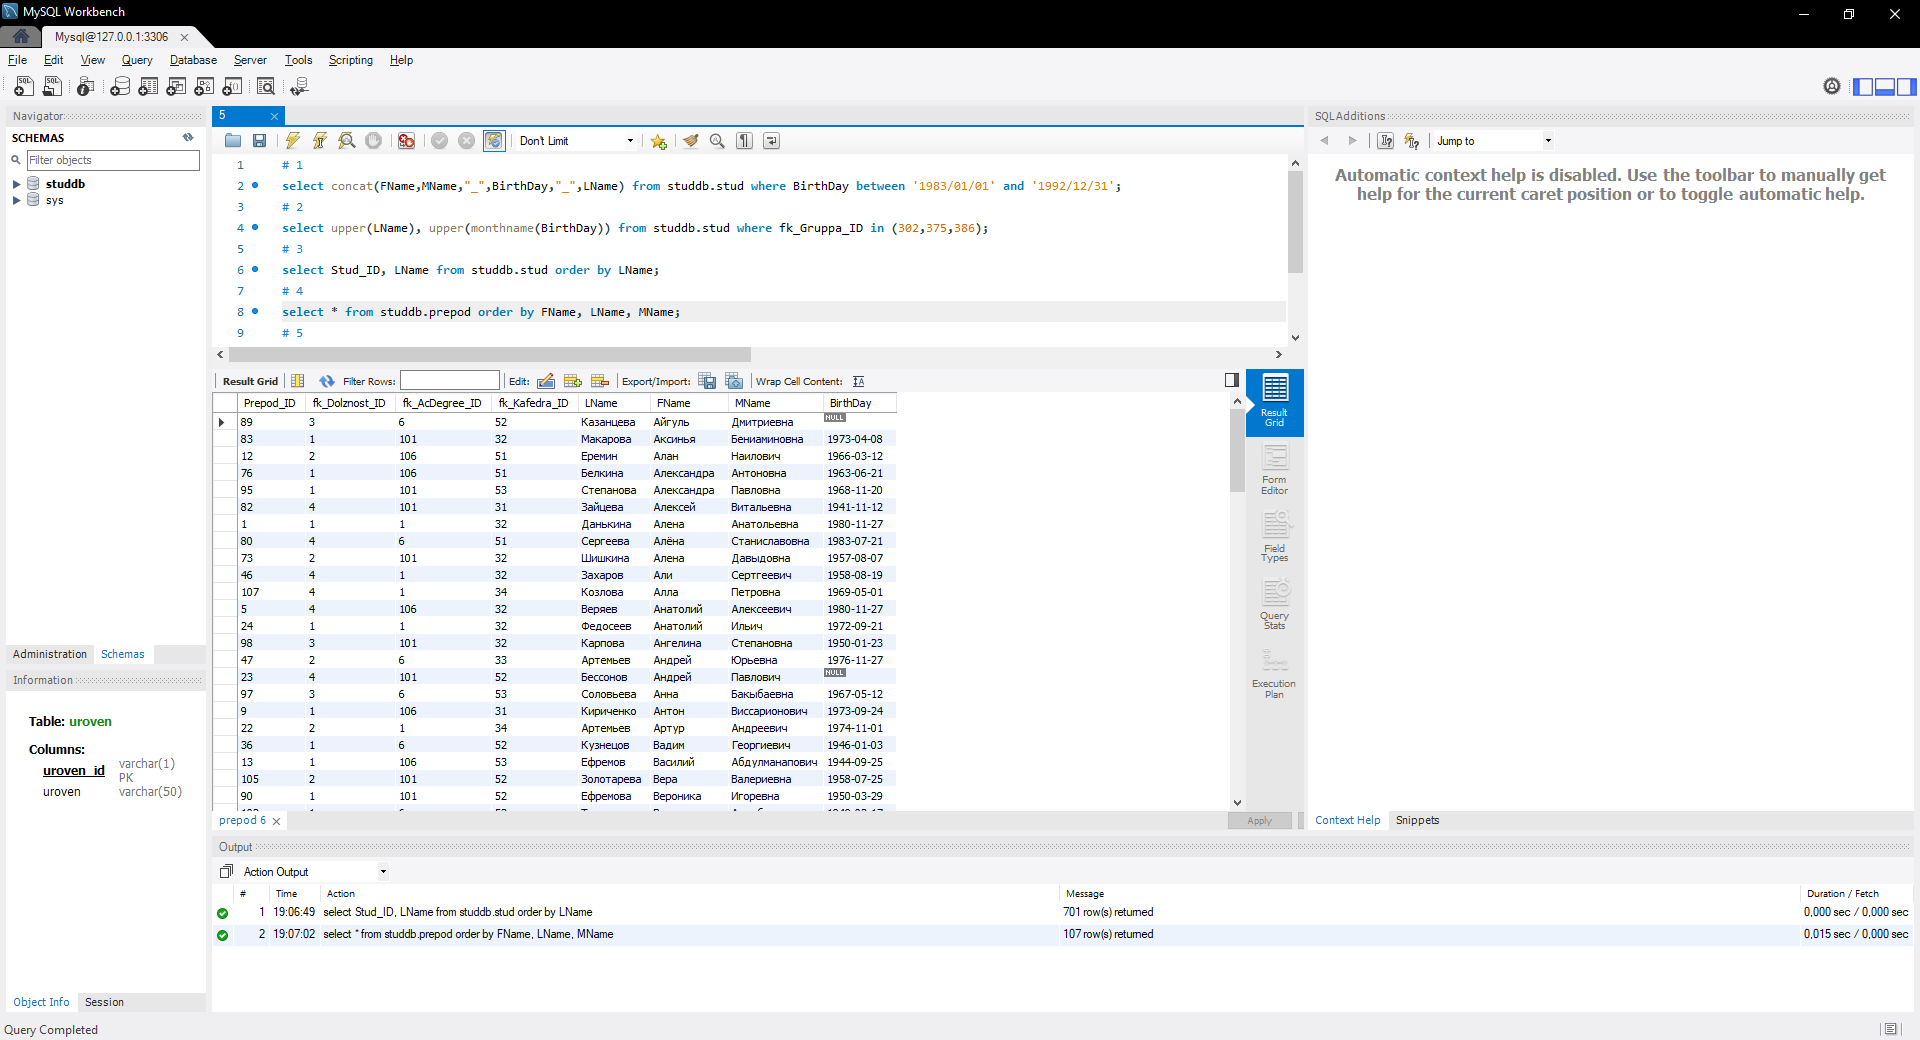
\includegraphics[width=\textwidth]{5-3.png}

\subsection{Вывести все сведения о студентах, родившихся с 10 по 31 июля 1989 года}
\begin{lstlisting}
select * from studdb.stud
where
	BirthDay between '1989/07/10' and '1989/07/31';
\end{lstlisting}
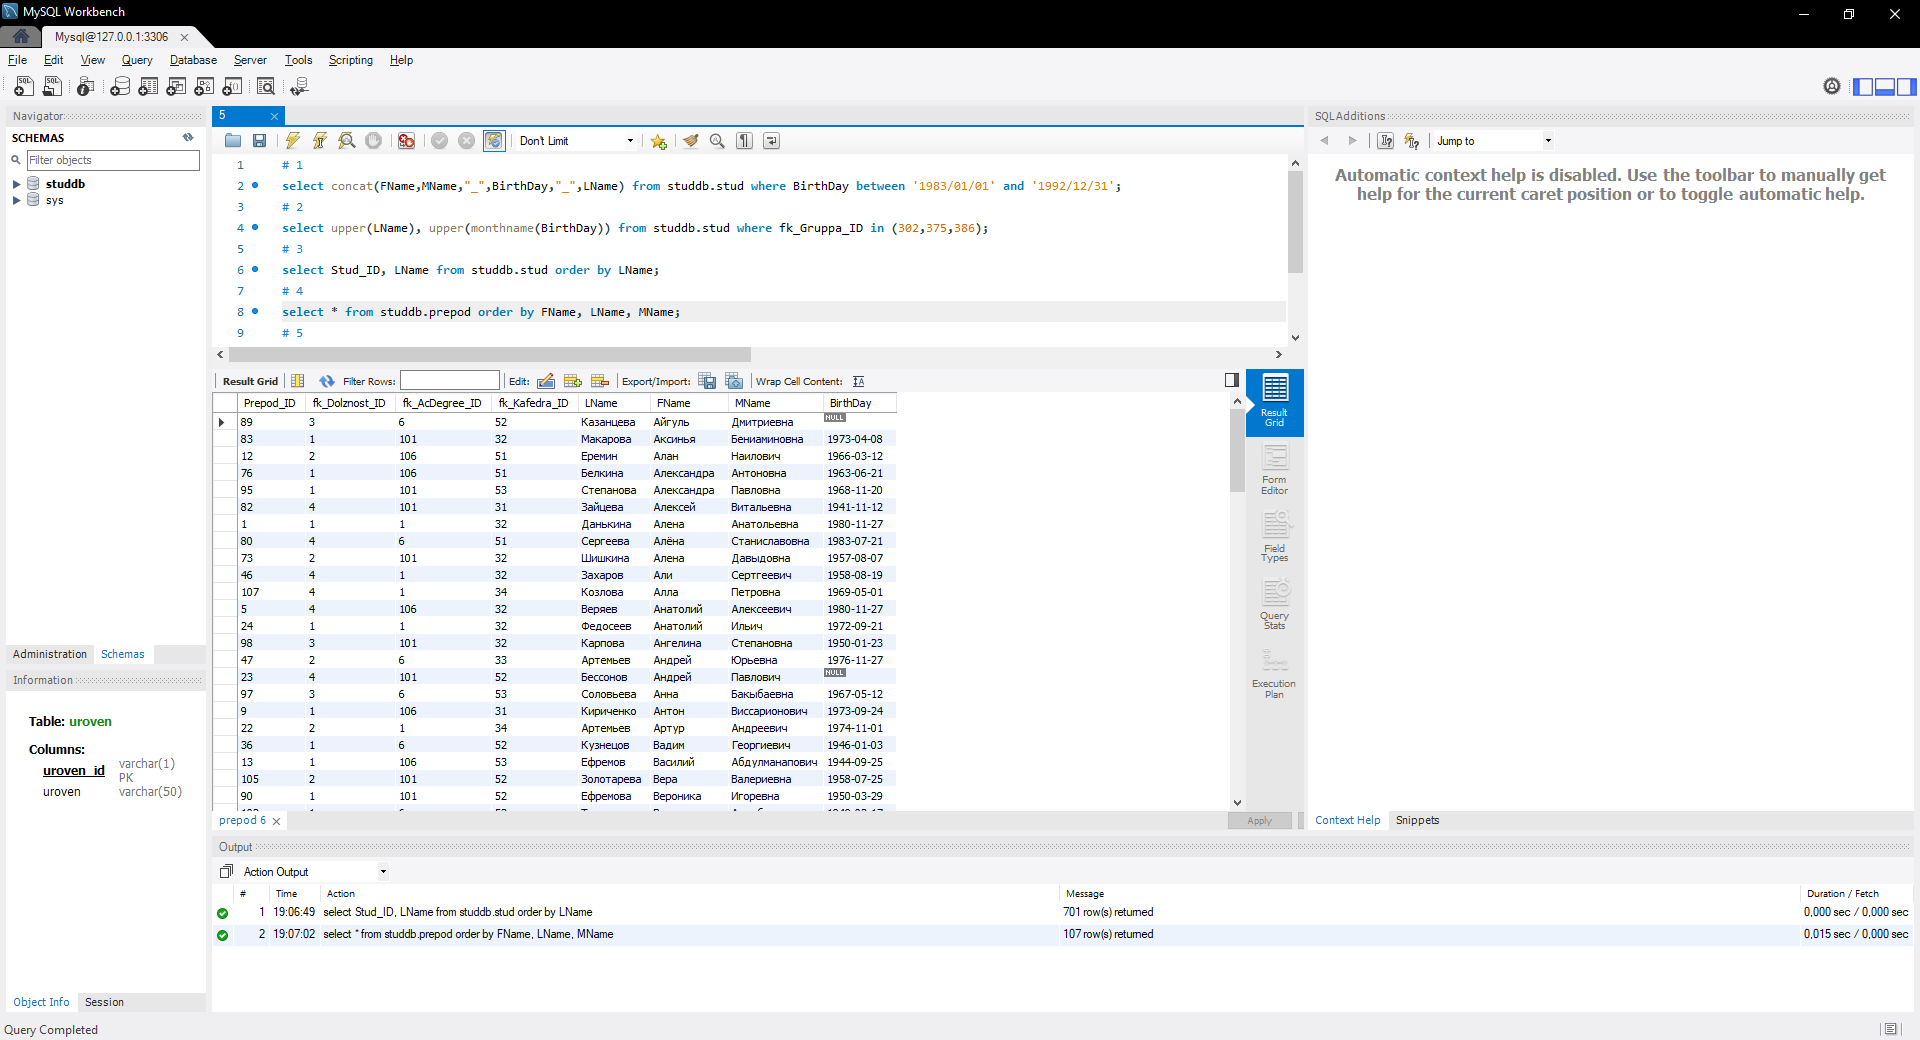
\includegraphics[width=\textwidth]{5-4.png}

\newpage
\section{Вывод о проделанной работе}
В ходе данной работы были изучены основы работы с типом данных Дата,Время, изучены базовые условия запросов. 

\end{document}